\chapter{MARCO TEÓRICO}\label{chap:marco}
\vskip 3.0ex

En este capítulo se presentan las definiciones de grafos, cliques maximales, y algunas métricas de clusterización, junto a codificaciones ocupadas en este trabajo.

\section{Grafos, cliques maximales y métricas de clusterización} \label{marco:grafoclique}
Se define un \textbf{grafo} $G = (V, E)$ como el conjunto finito de \textit{vértices} o \textit{nodos} $V$ y el conjunto de \textit{aristas} $E \subseteq V \times V$ (arcos). La expresión $V(G)$ representa el conjunto de sus vértices y $E(G)$ el conjunto de sus aristas. El \textit{orden} de un grafo corresponde al total de sus vértices $|V(G)|$, mientras que el \textit{tamaño} de un grafo corresponde al total de sus aristas $|E(G)|$. 

Dos vértices $v_{1}$ y $v_{2} \in V(G)$ son \textbf{adyacentes} o \textbf{vecinos} si $(v_{1}, v_{2}) \in E(G)$ y $v_{1} \neq v_{2}$.  Un grafo es \textbf{no dirigido} cuando la arista conlleva ambos sentidos, quiere decir que $(v_{1}, v_{2}) = (v_{2}, v_{1})$, ambos vértices son vecinos directos entre sí. Caso aparte son los grafos \textbf{dirigidos}, donde las aristas tienen un solo sentido, y $(v_{1}, v_{2}) \neq (v_{2}, v_{1})$. En este caso, $v_{2}$ es llamado \textbf{vecino directo} de $v_{1}$, mientras $v_{1}$ es llamado \textbf{vecino inverso o reverso} de $v_{2}$. Un \textbf{grafo denso} es aquel que su número de aristas es cercano al máximo. Este trabajo está enfocado a utilizar grafos no dirigidos y poco densos. 

El \textbf{grado de un vértice} $d(v)$ se define como la cantidad de vértices en $V(G)$ que son adyacentes con $v$. La \textbf{matriz de adyacencia} de un grafo $G$ corresponde a una matriz binaria cuadrada $|V(G)| \times |V(G)|$ donde cada bit representa si un par de vértices $v_{1}$ y $v_{2} \in V(G)$ son vecinos o no. En resumen, todos sus valores son ceros a menos que haya una arista entre dichos vértices.

\begin{figure}[b]
    	\centering
    	\begin{minipage}{0.45\textwidth}
    		\centering
    		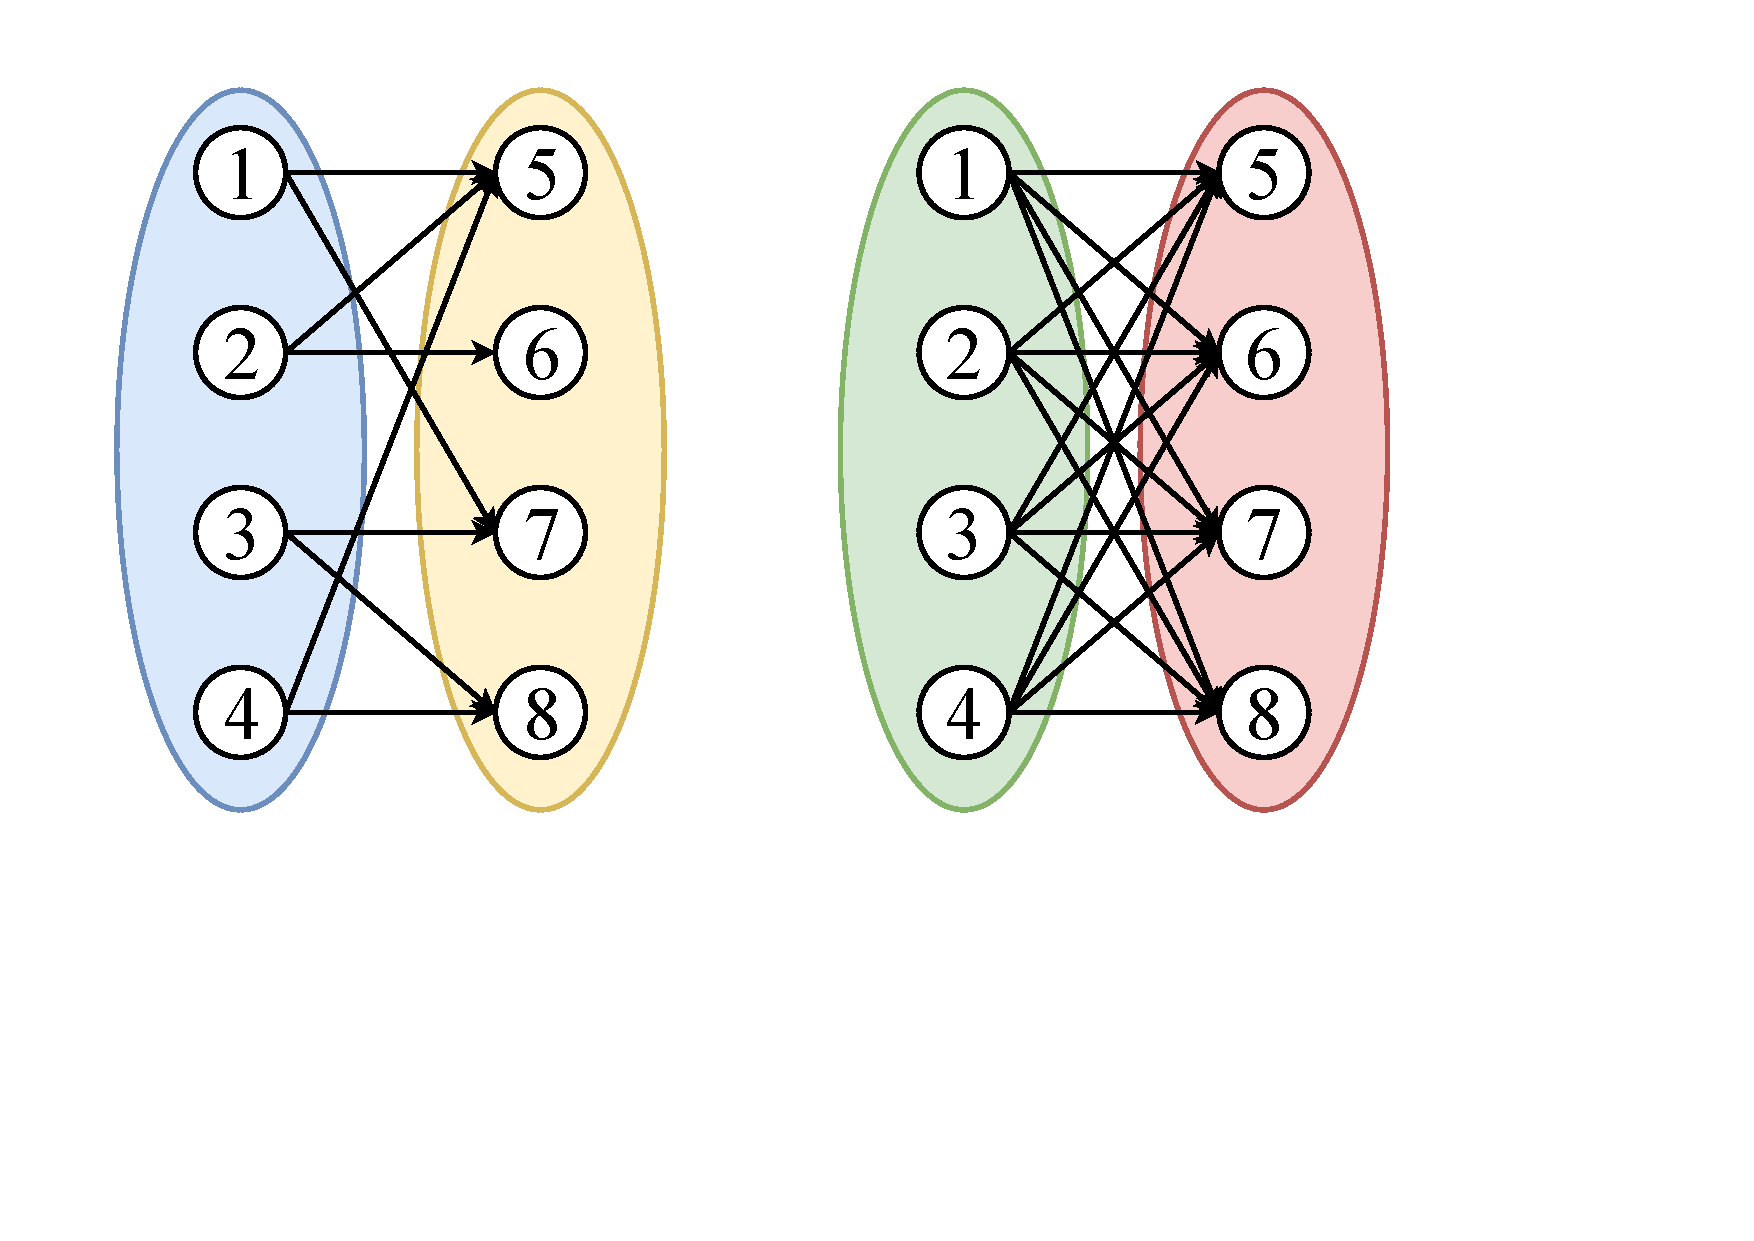
\includegraphics[scale=.3, clip,  trim=50 200 520 30]{img/graphs-bipartito.pdf}
    		
    		(a)
    	\end{minipage}
    	\begin{minipage}{0.45\textwidth}
    		\centering
    		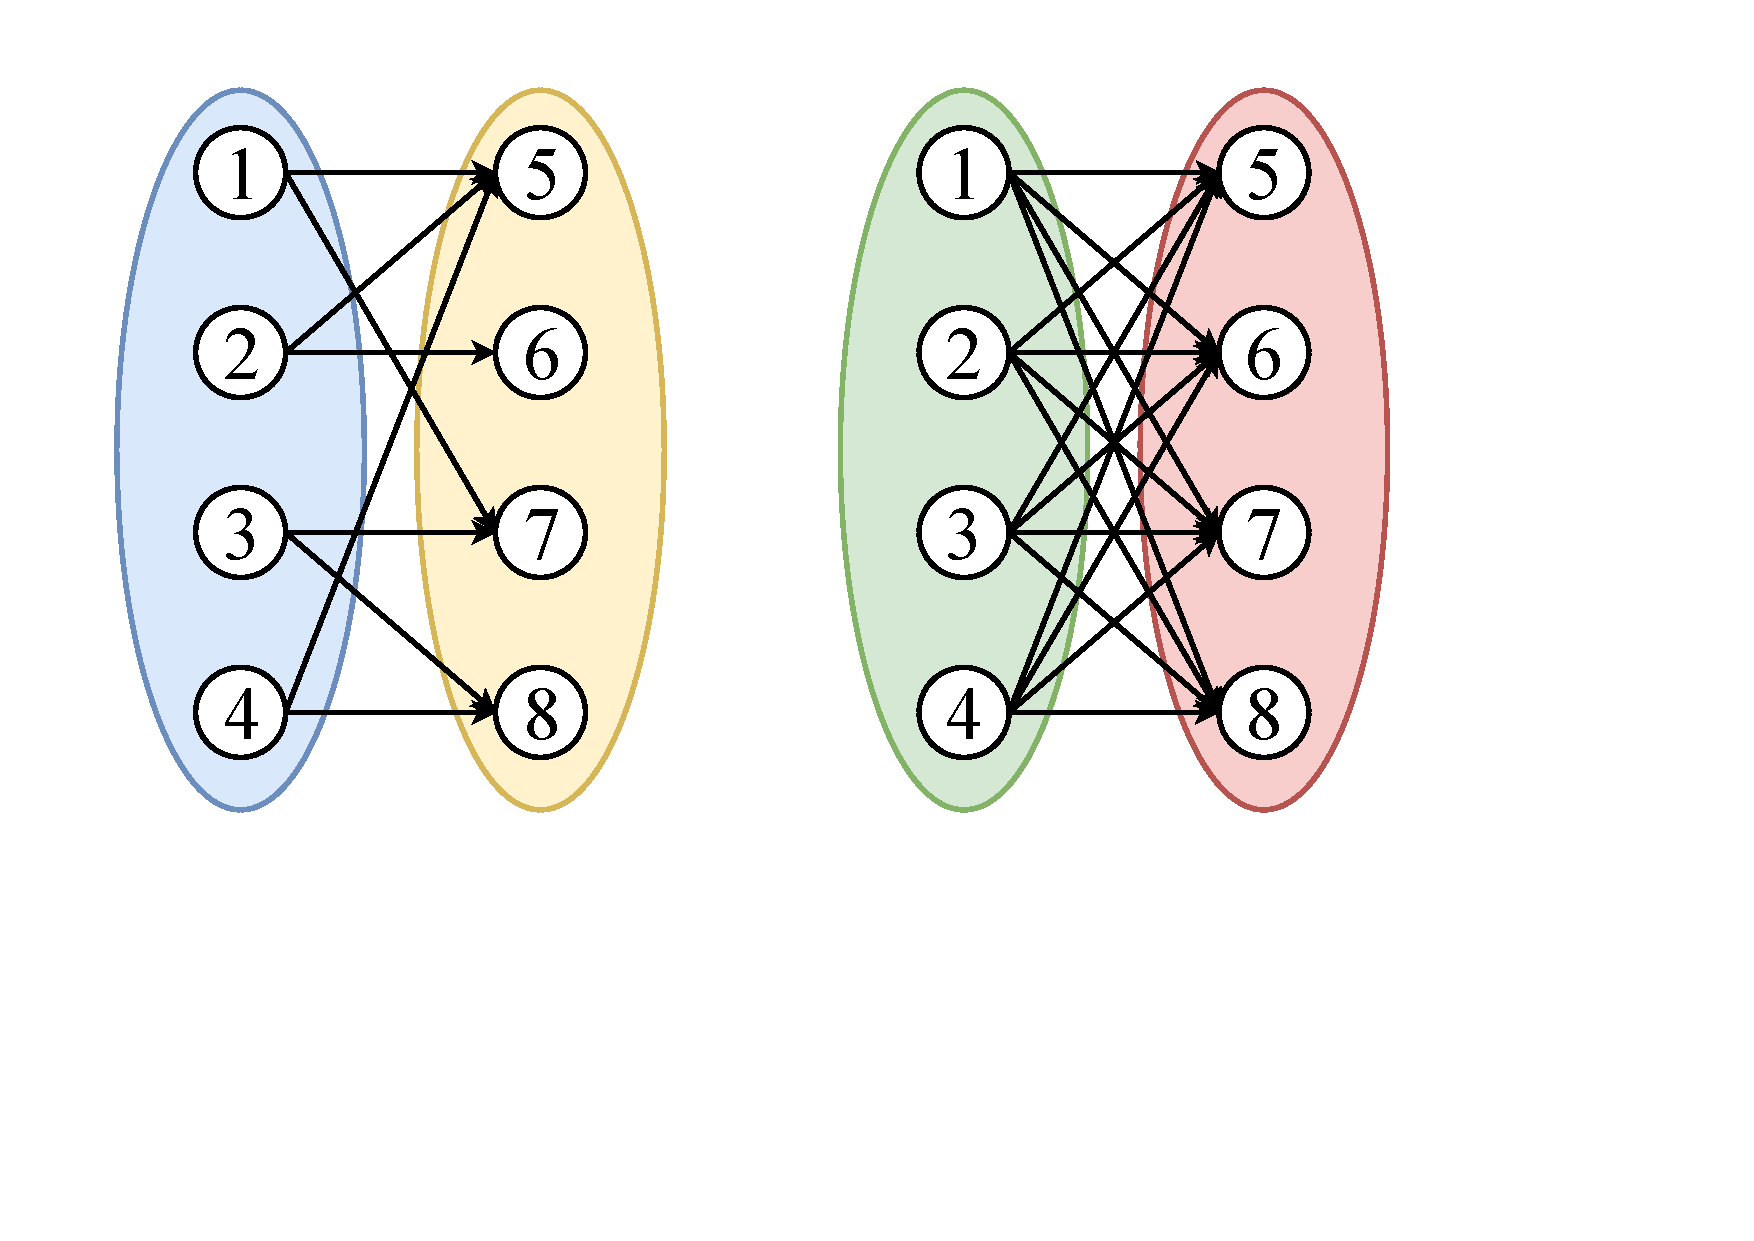
\includegraphics[scale=.3, clip, trim=400 200 170 30]{img/graphs-bipartito.pdf}
    		
    		(b)
    	\end{minipage}

    \caption{Ejemplo de grafos bipartitos. (a) Grafo bipartito. (b) Grafo bipartito completo o biclique.}
    \label{fig:bipartito}
\end{figure}


Un grafo \textbf{k-degenerate} es no dirigido, donde cada subgrafo tiene un vértice con grado a lo más \textbf{k}. El índice de \textbf{degeneracy} de un grafo, $D(G)$, es el menor valor \textbf{k} para el cual el grafo es \textbf{k-degenerate}.

Un grafo es \textbf{bipartito} cuando sus vértices se pueden separar en dos conjuntos separados $U$ y $W$, tal que se cumple $U \cup W = V$ y $U \cap W = \varnothing$. Un grafo es \textbf{bipartito completo} o \textbf{biclique}, cuando todos los vértices de un conjunto son vecinos directos de todos los vértices del otro conjunto. En la Figura~\ref{fig:bipartito} se ilustra un ejemplo de grafo bipartito y un biclique.


Un \textbf{clique} es un subgrafo donde todos los vértices son adyacentes entre sí, es decir, $\exists V' \subseteq V(G), \forall v_{1}, v_{2} \in V', (v_{1}, v_{2}) \in E(G) $. Un \textbf{clique maximal} no puede extenderse incluyendo otro vértice adyacente, es decir, no es subconjunto de otro clique más grande. En la Figura~\ref{fig:maxCliqueExample} se presenta ejemplo de un grafo y sus cliques maximales.

\begin{figure}
    	\centering
    	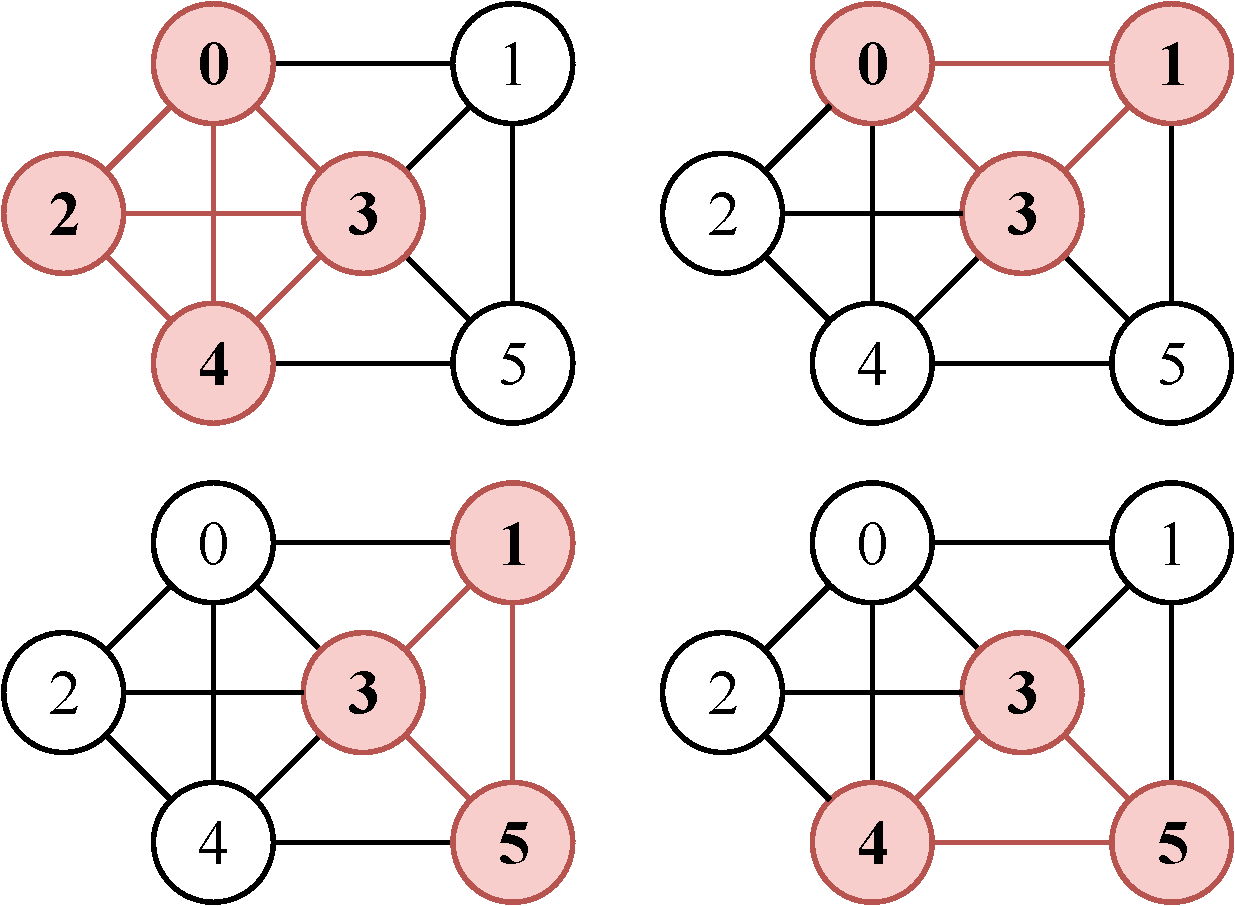
\includegraphics[width=0.5\linewidth]{img/maxCliqueExample.pdf}
    	
    \caption{Ejemplo de grafo y sus cliques maximales.}
    \label{fig:maxCliqueExample}
\end{figure}


Un \textbf{triángulo} es un subgrafo de tres vértices y tres aristas. Se define $\lambda(v)$ como la cantidad de triángulos donde participa un nodo $v$, y $\lambda(G)$ como la cantidad de triángulos de un grafo, y se calcula sumando el cálculo individual para cada vértice, y dividiendo el total en tres (por cada triángulo se cuentan 3 veces los vértices), como lo muestra la siguiente ecuación

\begin{equation}
	\lambda(G) = \dfrac{1}{3} \sum_{v \in V} \lambda(v) \label{eq:triangles}
\end{equation}

Un \textbf{triplete} es un subgrafo de tres vértices y dos aristas, donde las aristas comparten un vértice común. Se define $\tau(v)$ como la cantidad de tripletes donde $v$ es el vértice común, y $\tau(G)$ como la cantidad de tripletes de un grafo.

\begin{equation}
	\tau(G) = \sum_{v \in V} \tau(v) \label{eq:triplets}
\end{equation}

El \textbf{coeficiente de clusterización} de un vértice indica cuánto está conectado con sus vecinos, y se define como $c(v) =  \lambda(v) / \tau(v)$. El coeficiente de clusterización de un grafo ($C(G)$) es el promedio del coeficiente de todos los nodos del grafo, y se define como:

\begin{align}
	C(G) &= \dfrac{1}{|V'|} \sum_{v \in V'} c(v) \label{eq:CC} \\
	V' &= \{ v \in V | d(v) \geq 2 \} \nonumber
\end{align}

\noindent donde $V'$ es el conjunto de vértices con un grado mayor a dos. Su rango es entre $[0, 1]$, mientras más cercano a $1$ indica más conexión entre vértices.

La \textbf{transitividad} de un grafo ($T(G)$) es la probabilidad que un par de nodos adyacentes estén interconectados, y se define como:

\begin{equation}
	T(G) = \dfrac{3 \lambda(G)}{\tau(G)} \label{eq:T} 
\end{equation}

\noindent y su rango también va entre $[0, 1]$, siendo $1$ cuando todos los nodos están interconectados con todos.

Tanto el coeficiente de clusterización como la transitividad son métricas que permiten vislumbrar cuán conectados o clusterizados están los vértices de un grafo, y de sus ecuaciones se puede notar que están relacionados.

\section{Codificaciones}

Existen distintos tipos de codificaciones, según la aplicación. En esta sección se resumen algunas de relevancia para este trabajo, como algunos códigos universales o la codificación Huffman.

\subsection{Códigos universales}\label{sec:Ucoding}
Los códigos universales para enteros son un tipo de códigos que transforman enteros positivos en secuencias de bits, donde el largo de la secuencia final de bits tiene relación con el entero a codificar. Existen varios códigos de este tipo, algunos son:

\begin{itemize}
	\item \textbf{Código unario}: Se representa un entero $x$ por una secuencia de $1^{x-1}0$, donde el $0$ indica el término de la secuencia. Por ejemplo, el número $5$ se representa por la secuencia $111110$. Este código no es muy eficiente por si solo, pero se usa de base para otro tipo de códigos.
	
	\item \textbf{Código gamma ($\gamma$)}: Se representa un entero $x$ en un par concatenado de \textit{largo} y \textit{offset}. \textit{Offset} es la representación binaria de $x$, pero sin el primer 1. Por ejemplo, para $x=5$ su representación binaria es $101$, por tanto su \textit{offset} es $01$. \textit{Largo} codifica el largo de \textit{offset} en código unario. Para $x=5$, el largo de \textit{offset} es 2 bits, por tanto \textit{largo} es $110$. Concatenando ambas, el código $\gamma$ para $x=5$ es $11001$.
	
	\item \textbf{Código delta ($\delta$)}: Este código es una extensión del código $\gamma$ para enteros largos. Básicamente hacen lo mismo, pero el \textit{largo} lo representan en código $\gamma$ en vez de código unario. El código $\delta$ para $x=5$ es $10001$.
\end{itemize}

\subsection{Codificación Huffman}\label{sec:huffman}
Una codificación muy usada es la propuesta por Huffman\cite{huffman1952method}, que retorna códigos prefijo de largo variable. Su conversión se basa en la frecuencia de los símbolos en la secuencia de entrada, codificando los más frecuentes con menos bits. Para recuperar la secuencia original, esta representación requiere tanto la secuencia codificada junto a un vocabulario de símbolos.

Una codificación binaria de largo fijo, le asigna la misma cantidad de bits a todos los símbolos por codificar. Una de largo variable le asigna menos bits a los símbolos más frecuentes, y más bits a los menos frecuentes, cuidando que las secuencias binarias cortas no sean prefijos de las más largas. La Figura~\ref{fig:fixedVarLength} se tiene la frecuencia de seis símbolos en una secuencia de 100.000 caracteres, y se comparan ambos códigos. Para el caso de largo fijo, se requieren 3 bits por cada símbolo en la secuencia, un total de 300.000 bits. Para el caso de largo variable, el símbolo más frecuente \texttt{a} requiere un bit, y los menos frecuentes requieren 4 bits. Así, la secuencia requiere:

\begin{align*}
	(45 \cdot 1 + 13 \cdot 3 + 12 \cdot 3 + 16 \cdot 3 + 9 \cdot 4 + 5 \cdot 4) \cdot \textrm{1.000} = \textrm{224.000 bits}
\end{align*}

\noindent lo que significa una reducción cercana al $20\%$. 

Un código prefijo es aquel donde ninguna palabra codificada es usada como prefijo de otra. Estos códigos son simples de decodificar, basta con comenzar el proceso desde el primer bit hasta encontrar una de las posibles codificaciones, traducirla a su valor original, y seguir con el resto de bits codificados. Siguiendo el ejemplo, la secuencia $001011101$ se identifica como $0 \cdot 0 \cdot 101 \cdot 1101$, y se traduce como \texttt{aabe}.

Para agilizar la búsqueda, el código prefijo se puede representar como un árbol binario, donde los nodos hojas son los caracteres codificados. Siguiendo cada bit de la secuencia, se puede ir avanzando por el árbol hasta llegar a un nodo hoja, y así llegar al valor buscado. En la Figura~\ref{fig:fixVarTrees} se ilustran los árboles de las codificaciones de la Figura~\ref{fig:fixedVarLength}, en (a) el correspondiente a código de largo fijo, y en (b) el de largo variable.

 \begin{figure}[b]
    	\centering
    
    \begin{tabular}{l|cccccc}
    		& a & b & c & d & e & f \\
    		\midrule
    		Frecuencia (en miles) & 45 & 13 & 12 & 16 & 9 & 5 \\
    		Código largo fijo & 000 & 001 & 010 & 011 & 100 & 101 \\
    		Código largo variable & 0 & 101 & 100 & 111 & 1101 & 1100 \\
    \end{tabular}

    \caption{Ejemplo de códigos de largo fijo y largo variable.}
    \label{fig:fixedVarLength}
\end{figure}


\begin{figure}[b]
    	\centering
    	\begin{minipage}{0.45\textwidth}
    		\centering
    		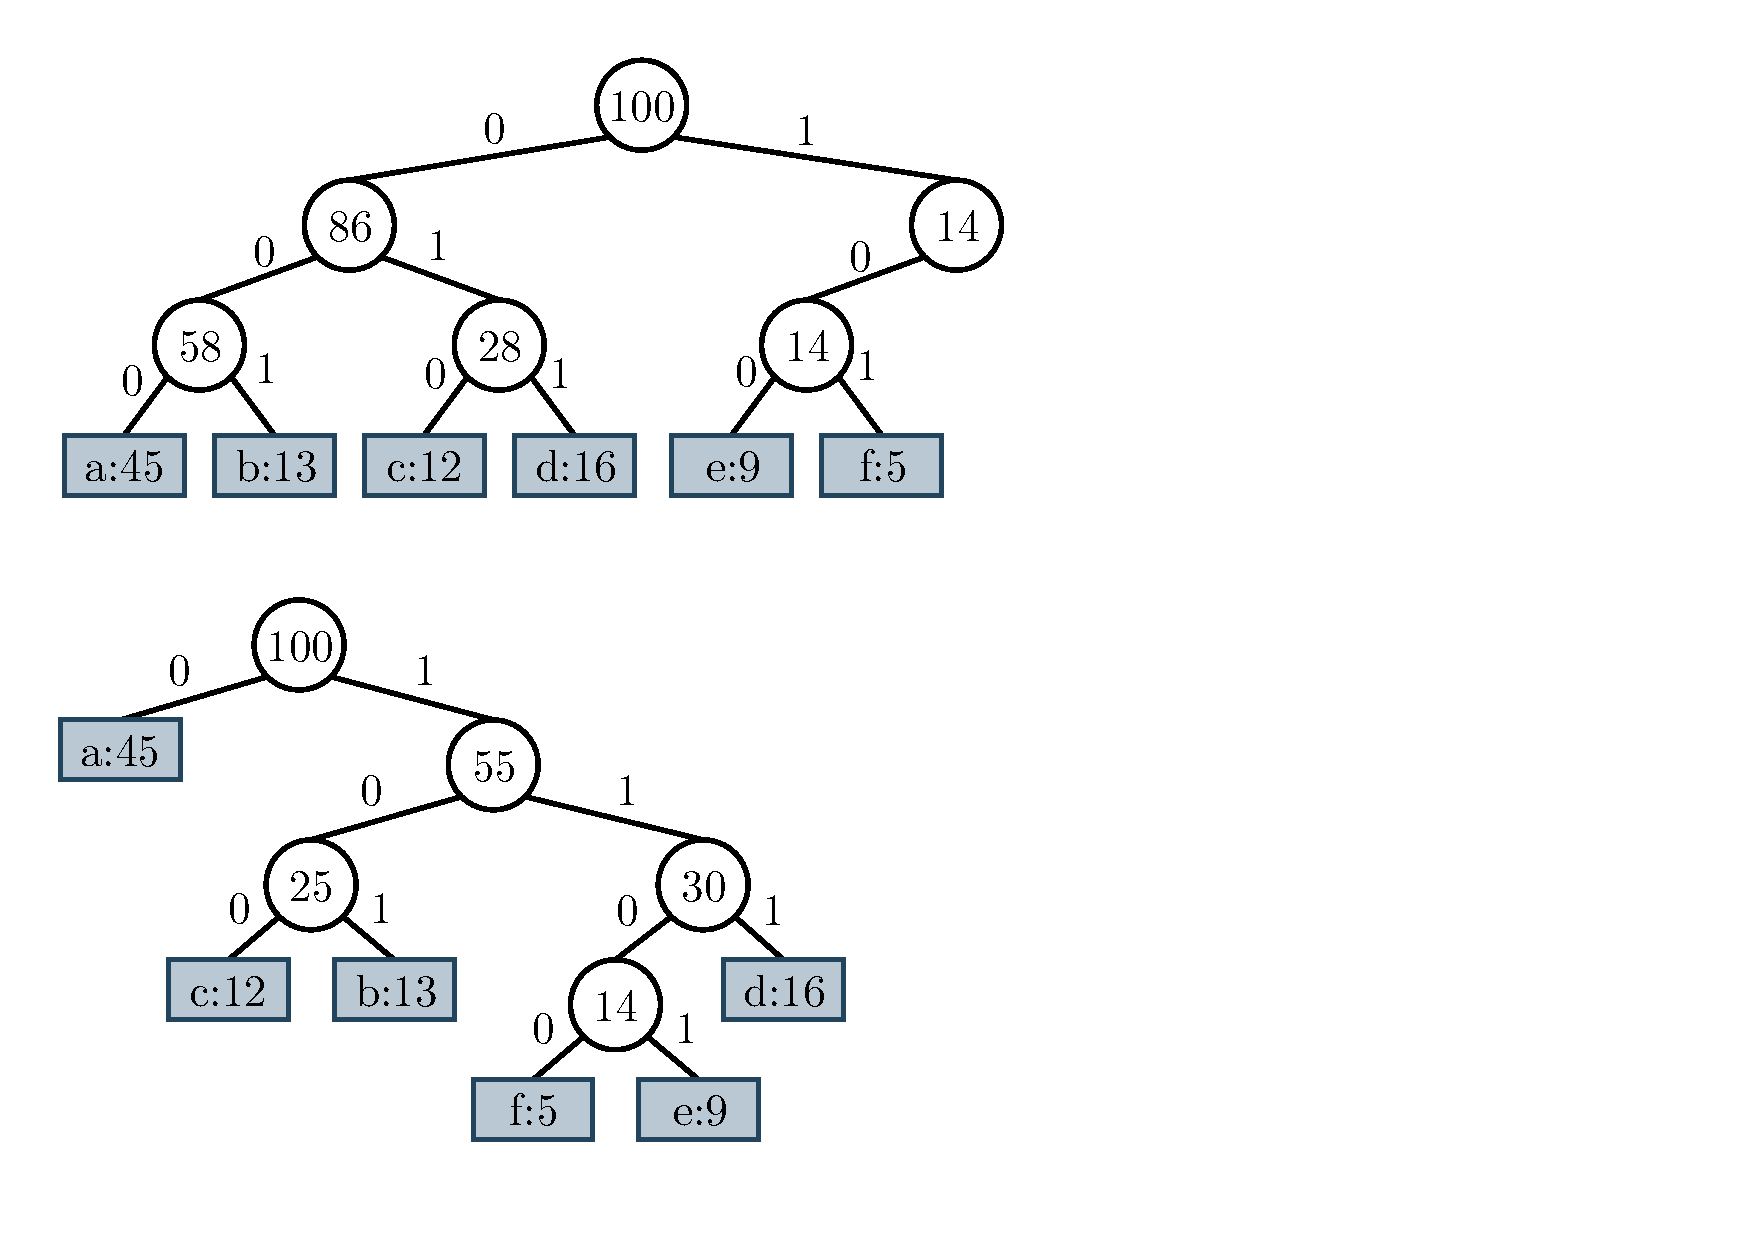
\includegraphics[scale=.45, clip,  trim=20 350 350 20]{img/graphs-fixVarTrees.pdf}
    		
    		(a)
    	\end{minipage}
    	\begin{minipage}{0.45\textwidth}
    		\centering
    		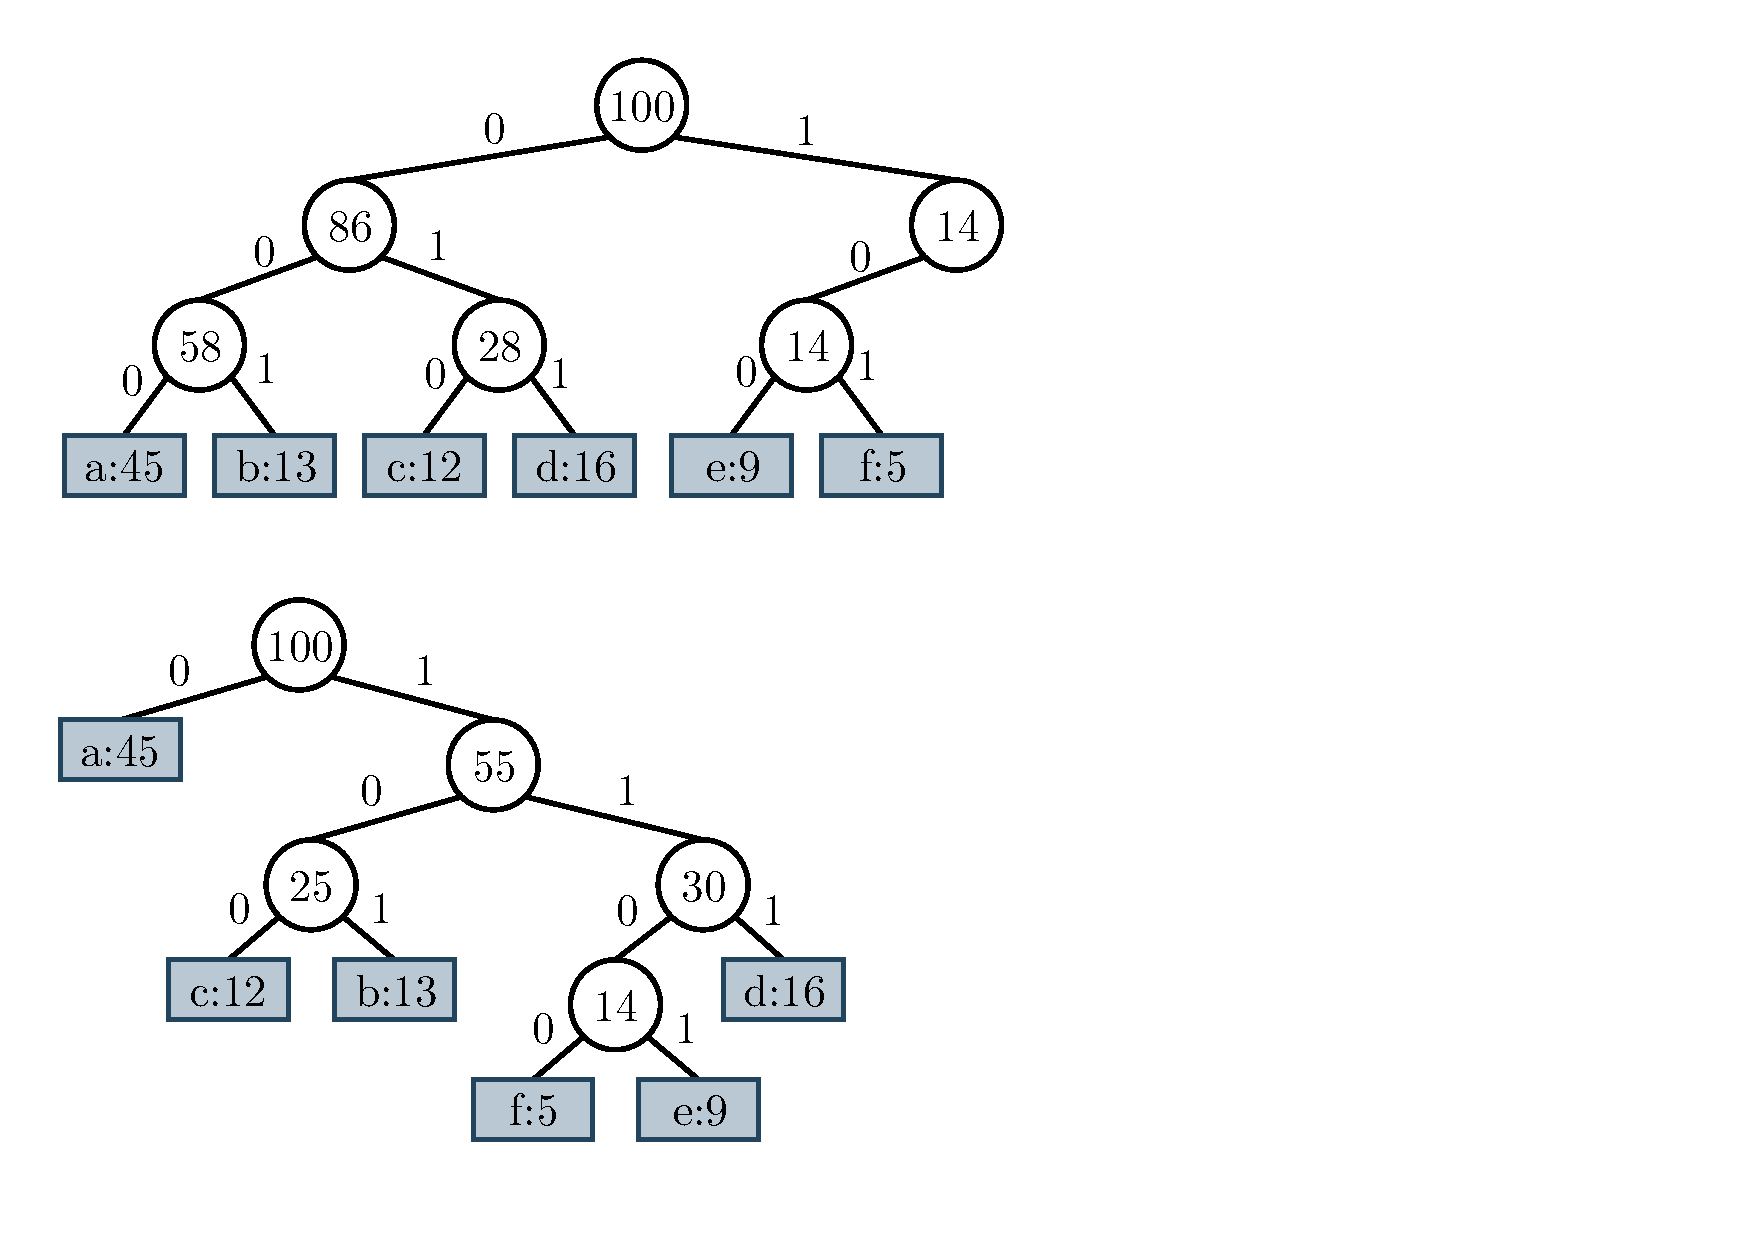
\includegraphics[scale=.45, clip, trim=20 40 430 280 ]{img/graphs-fixVarTrees.pdf}
    		
    		(b)
    	\end{minipage}

    \caption{Árboles correspondientes a los códigos de la Figura~\ref{fig:fixedVarLength}. (a)~Árbol para código de largo fijo. (b)~Árbol para código de largo variable.}
    \label{fig:fixVarTrees}
\end{figure}


La codificación Huffman aprovecha todo lo anterior, utilizando una heurística \textit{greedy} para la construcción de su estructura y su compresión final. Asumiendo que se tiene una secuencia $C$ de $n$ caracteres, y que cada carácter $c \in C$ tiene una frecuencia $f[c]$ en $C$. El algoritmo crea un árbol desde los nodos hojas hacia el nodo raíz, inicialmente con $|C|$ hojas, y ejecutando $|C| - 1$ conexiones para llegar al árbol final. Luego identifica los dos elementos menos frecuentes y los conecta a un nuevo elemento, con frecuencia igual a la suma de ambos. Esto continúa hasta que todos los nodos hojas están conectados al árbol. En la Figura~\ref{fig:huffman2} se ilustra este proceso para la secuencia ejemplo de la Figura~\ref{fig:fixVarTrees}(b), y a continuación se detalla el proceso:

\begin{enumerate}
	\item \textbf{Figura~\ref{fig:huffman2}(a)}: Se crean los $|C| = 6$ nodos hoja para cada carácter.
	\item \textbf{Figura~\ref{fig:huffman2}(b)}: Se identifican los dos nodos de caracteres menos frecuentes, $f$ con $f[f] = 5$ y $e$ con $f[e] = 9$ (en miles), y se conectan a un nuevo nodo con frecuencia $5 + 9 = 14$.
	\item \textbf{Figura~\ref{fig:huffman2}(c)}: Los siguientes nodos menos frecuentes son $c$ con $f[c] = 12$ y $b$ con $f[b] = 13$, y se conectan a otro nodo nuevo con frecuencia $12 + 13 = 25$.
	\item \textbf{Figura~\ref{fig:huffman2}(d)}: El nodo creado que conecta $f$ con $e$ posee la menor frecuencia ($14$), y junto al nodo $d$ con $f[d] = 16$ se conectan en un nuevo nodo con frecuencia $14 + 16 = 30$.
	\item \textbf{Figura~\ref{fig:huffman2}(e)}: Para juntar a los nuevos nodos de menor frecuencia, $25$ y $30$ respectivamente, se crea un nuevo nodo con frecuencia $25 + 30 = 55$.
	\item \textbf{Figura~\ref{fig:huffman2}(f)}: Finalmente, se conecta el último nodo hoja restante, $a$ con $f[a] = 45$, con el reciente nodo creado de frecuencia $55$, mediante el nodo raíz con frecuencia $45 + 55 = 100$, confirmando la correcta creación del árbol.
\end{enumerate}

Se visualiza que se crearon $|C| - 1 = 6 - 1 = 5$ nodos para conectar todo el árbol. Con este resultado, se puede reconstruir de manera secuencial una secuencia codificada, simplemente recorriendo el árbol desde el nodo raíz hasta llegar a un nodo hoja, sustituir esa subsecuencia de bits por el valor de dicho nodo, y continuar con el resto de la secuencia de igual manera hasta el final. Retomando el ejemplo de secuencia $001011101$, en la Figura~\ref{fig:huffmanBack} se visualizan los tres casos a decodificar: en (a) los primeros bits $0$ llegan al nodo hoja de \texttt{a}, en (b) la secuencia $101$ llega al nodo \texttt{b}, y en (c) la secuencia $1101$ llega al nodo \texttt{e}, dando en (d) la equivalencia entre bits y caracteres con resultado \texttt{aabe}.

%\begin{figure}%[b]
    	\centering
    	\begin{minipage}{0.45\textwidth}
    		\centering

		\textbf{\large \textcolor{color3}{3}\textcolor{color2}{2}\textcolor{color3}{3}\textcolor{color3}{3}\textcolor{color1}{1}\textcolor{color2}{2}\textcolor{color3}{3}\textcolor{color1}{1}\textcolor{color3}{3}}
    		
    		(a)
		\vspace{10mm}  		
    		
    		\textbf{\large \textcolor{color3}{1}\textcolor{color2}{01}\textcolor{color3}{1}\textcolor{color3}{1}\textcolor{color1}{00}\textcolor{color2}{01}\textcolor{color3}{1}\textcolor{color1}{00}\textcolor{color3}{1}}
    		
    		(b)
    	\end{minipage}
    	\begin{minipage}{0.45\textwidth}
    		\centering
    		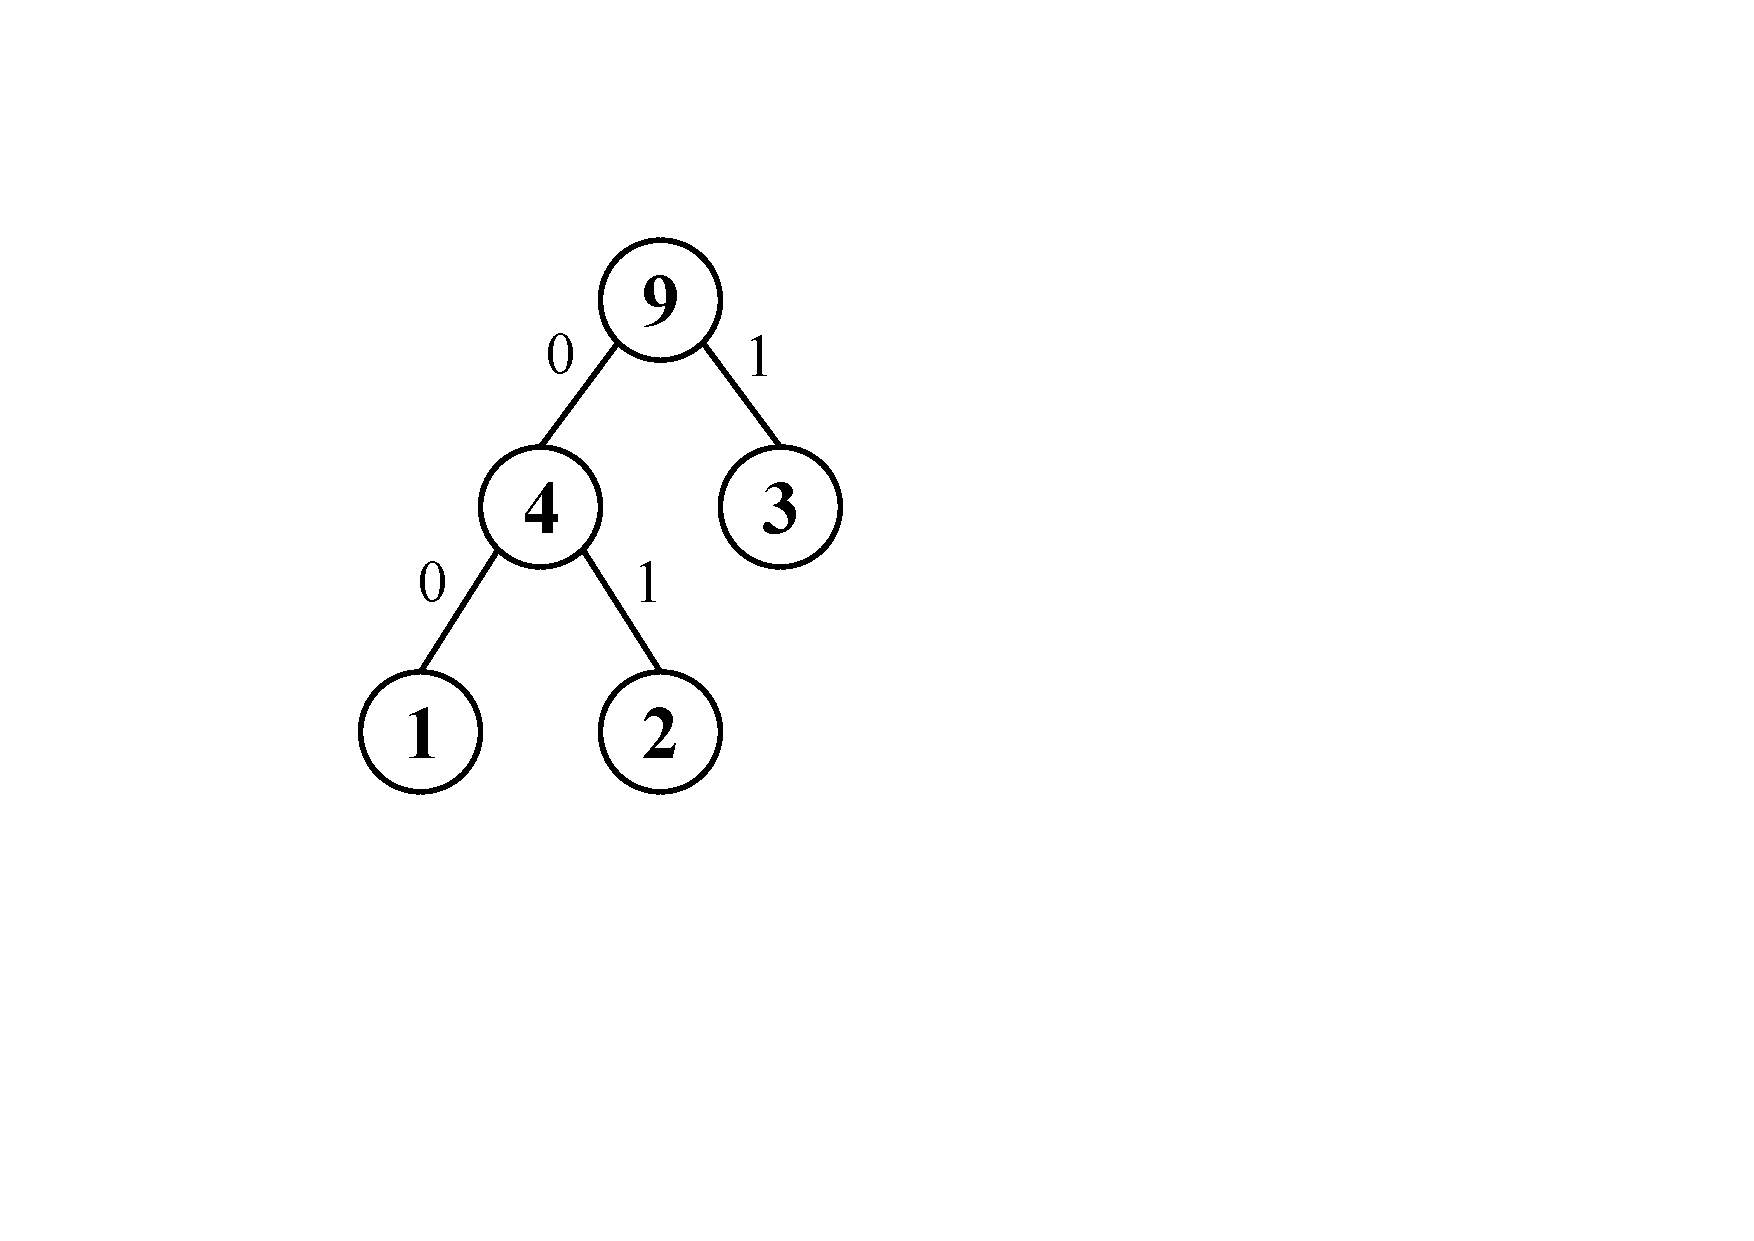
\includegraphics[scale=.4, clip, trim=160 200 410 100]{img/graphs-huffman.pdf}
    		
    		(c)
    	\end{minipage}

    \caption{Ejemplo de codificación Huffman. (a) Secuencia de entrada. (b) Secuencia de salida. (c) Diagrama de vocabulario en árbol binario.}
    \label{fig:huffman}
\end{figure}

\begin{figure}
    	\centering
    	\begin{minipage}{1\textwidth}
    		\centering
    		\begin{minipage}{0.45\textwidth}
    			\centering
    			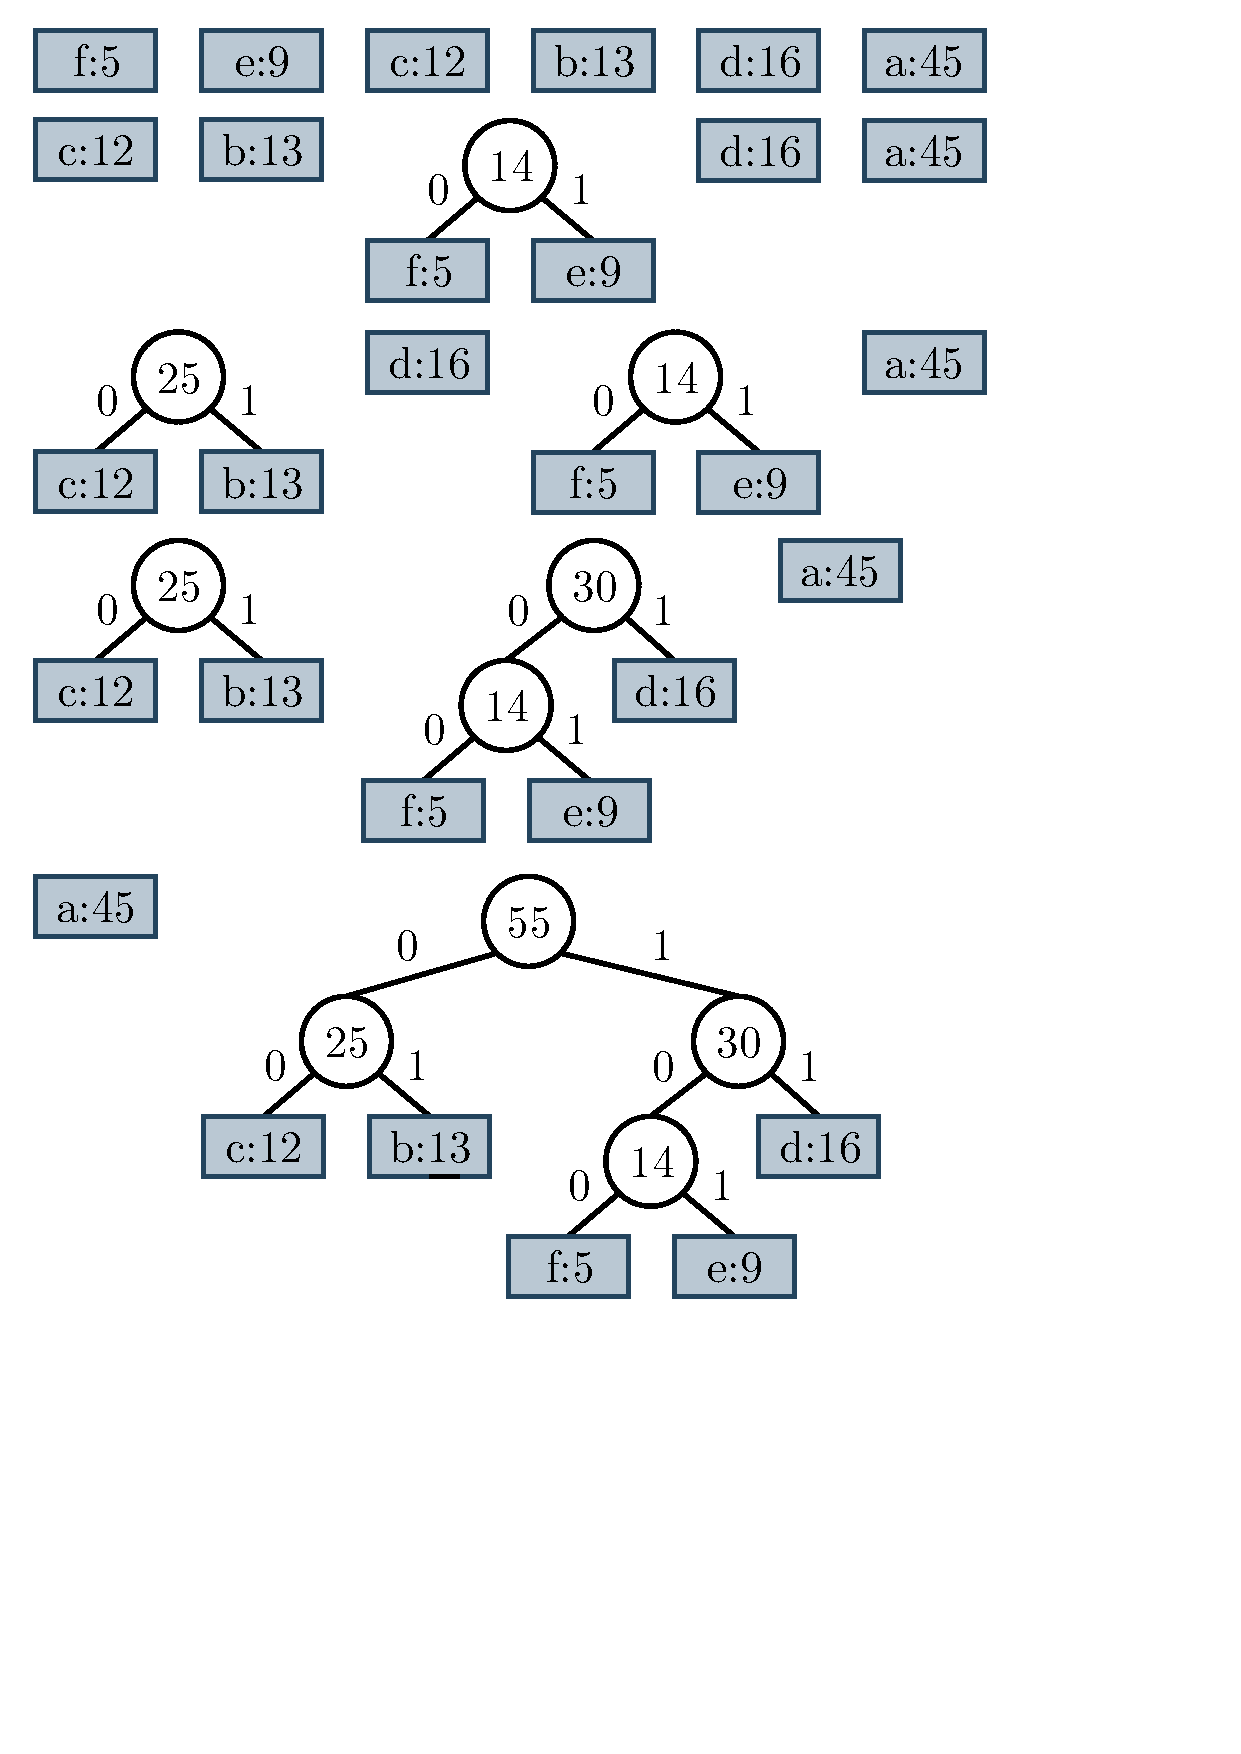
\includegraphics[scale=.45, clip, trim=16 790 120 10]{img/graphs-huffman2.pdf}
    			
    			(a)
    		\end{minipage}
    		\begin{minipage}{0.45\textwidth}
    			\centering
    			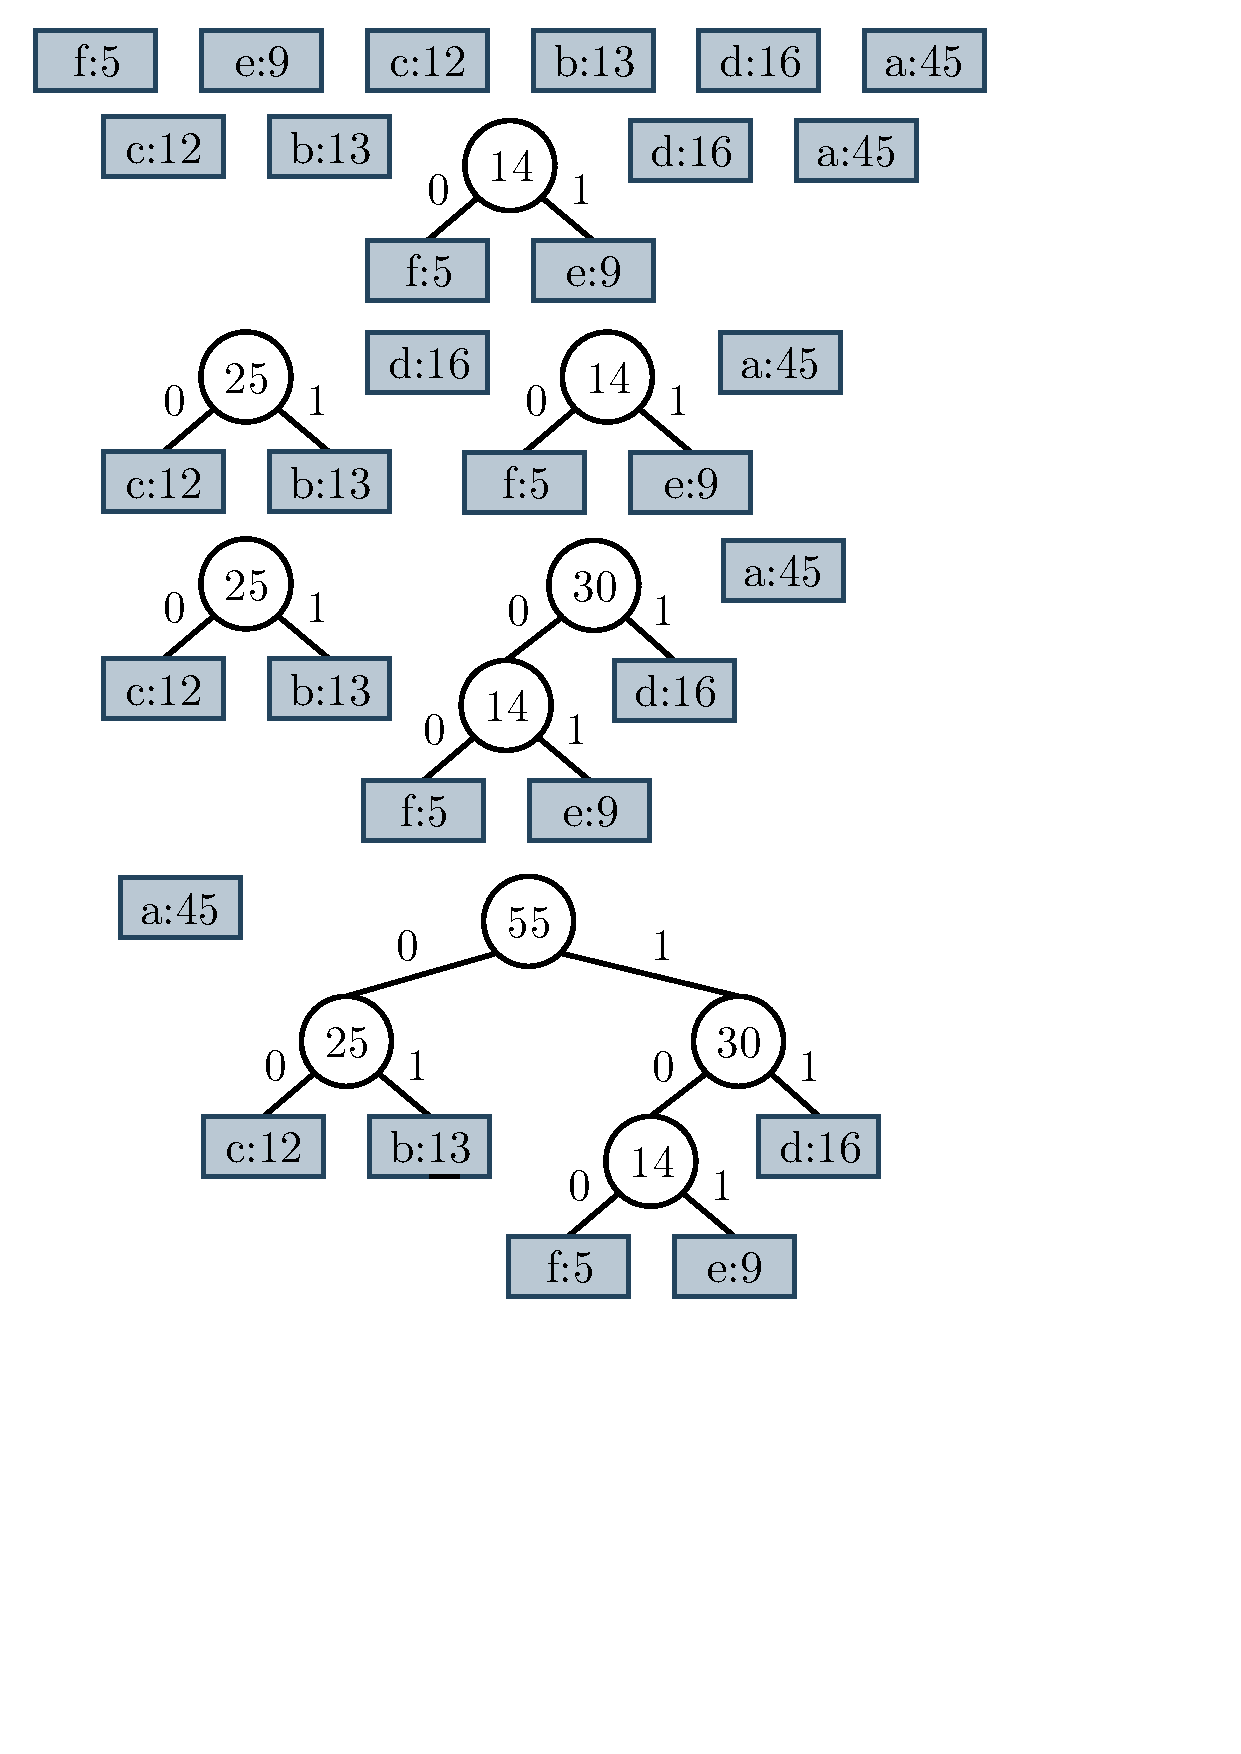
\includegraphics[scale=.45, clip, trim=40 690 150 50]{img/graphs-huffman21.pdf}

    			(b)
    		\end{minipage}  		
    	\end{minipage}
    	
    	\begin{minipage}{1\textwidth}
    		\centering
    		\begin{minipage}{0.45\textwidth}
    			\centering
    			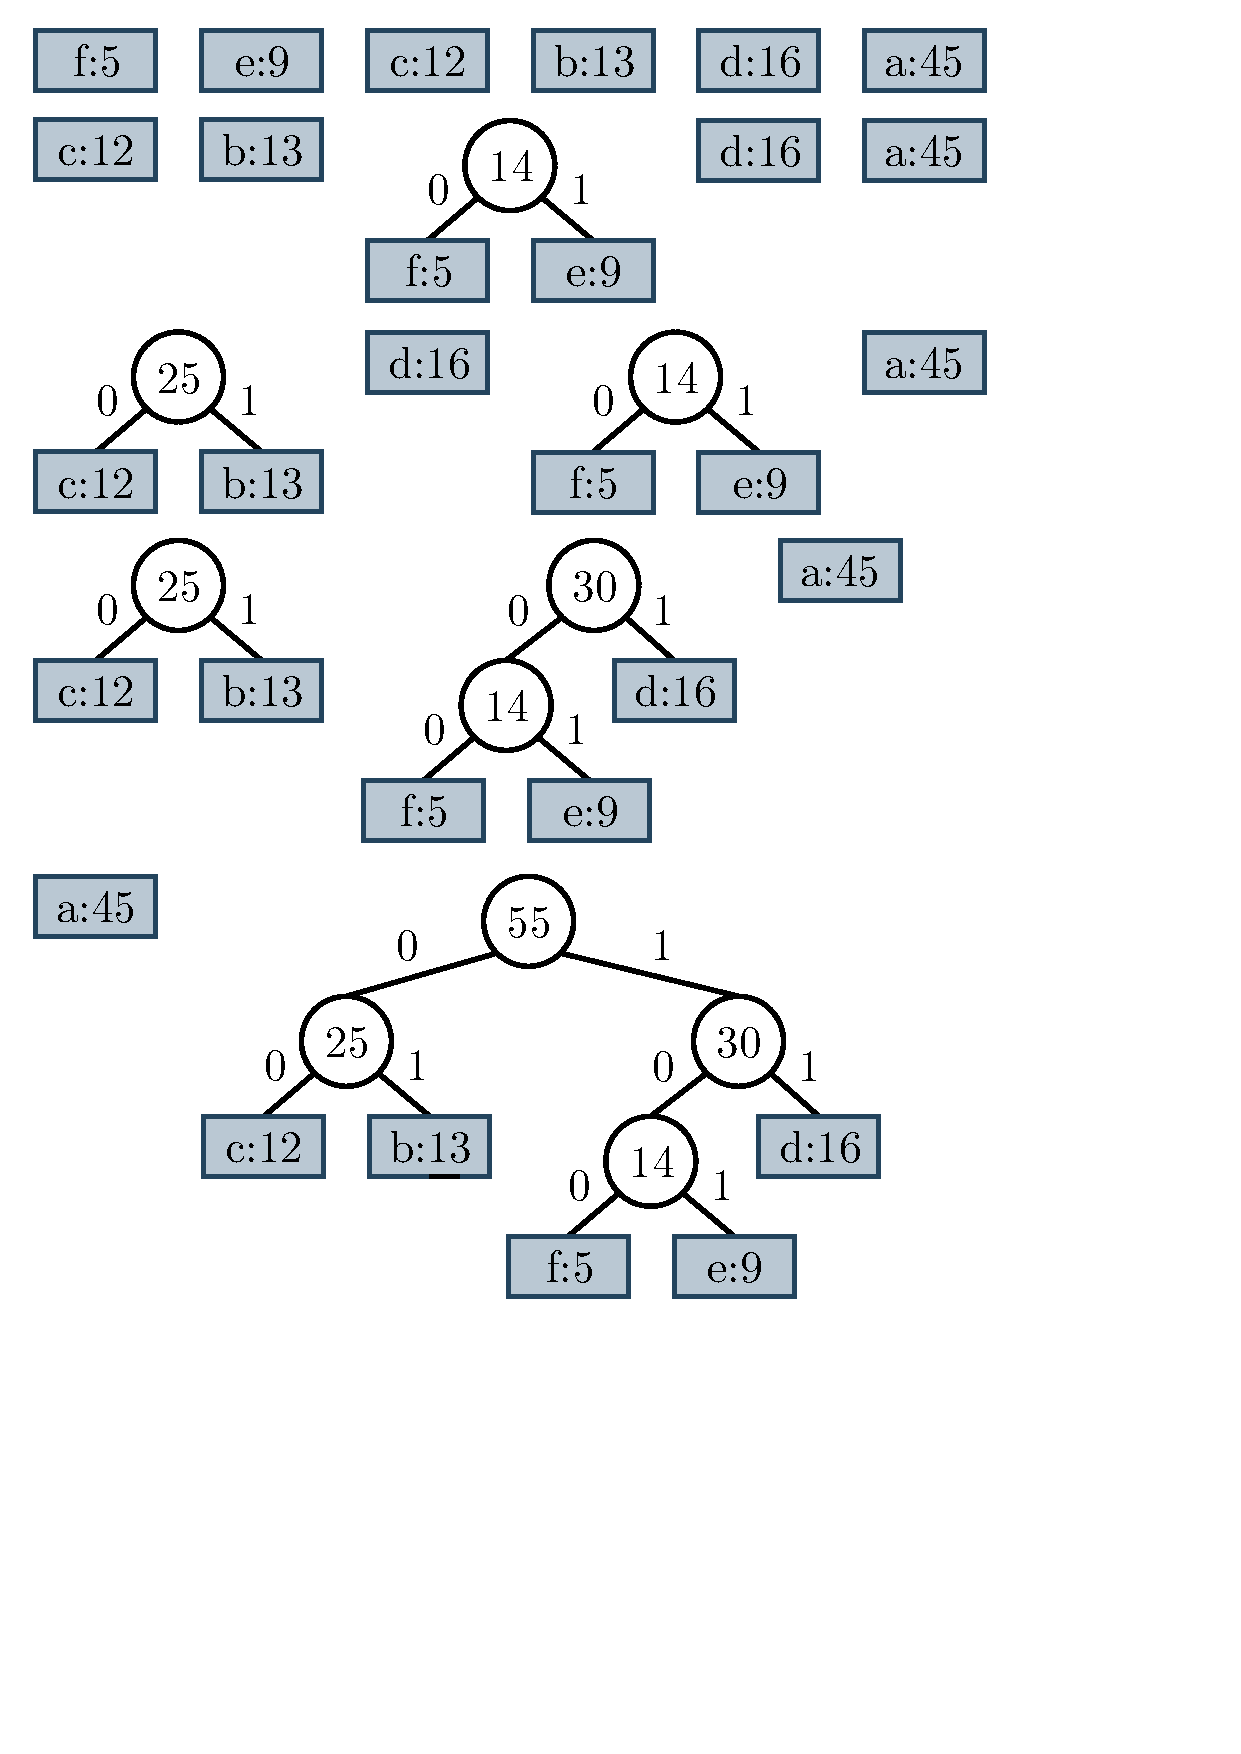
\includegraphics[scale=.4, clip, trim=10 590 120 150]{img/graphs-huffman2.pdf}
    			
    			(c)
    		\end{minipage}
    		\begin{minipage}{0.45\textwidth}
    			\centering
    			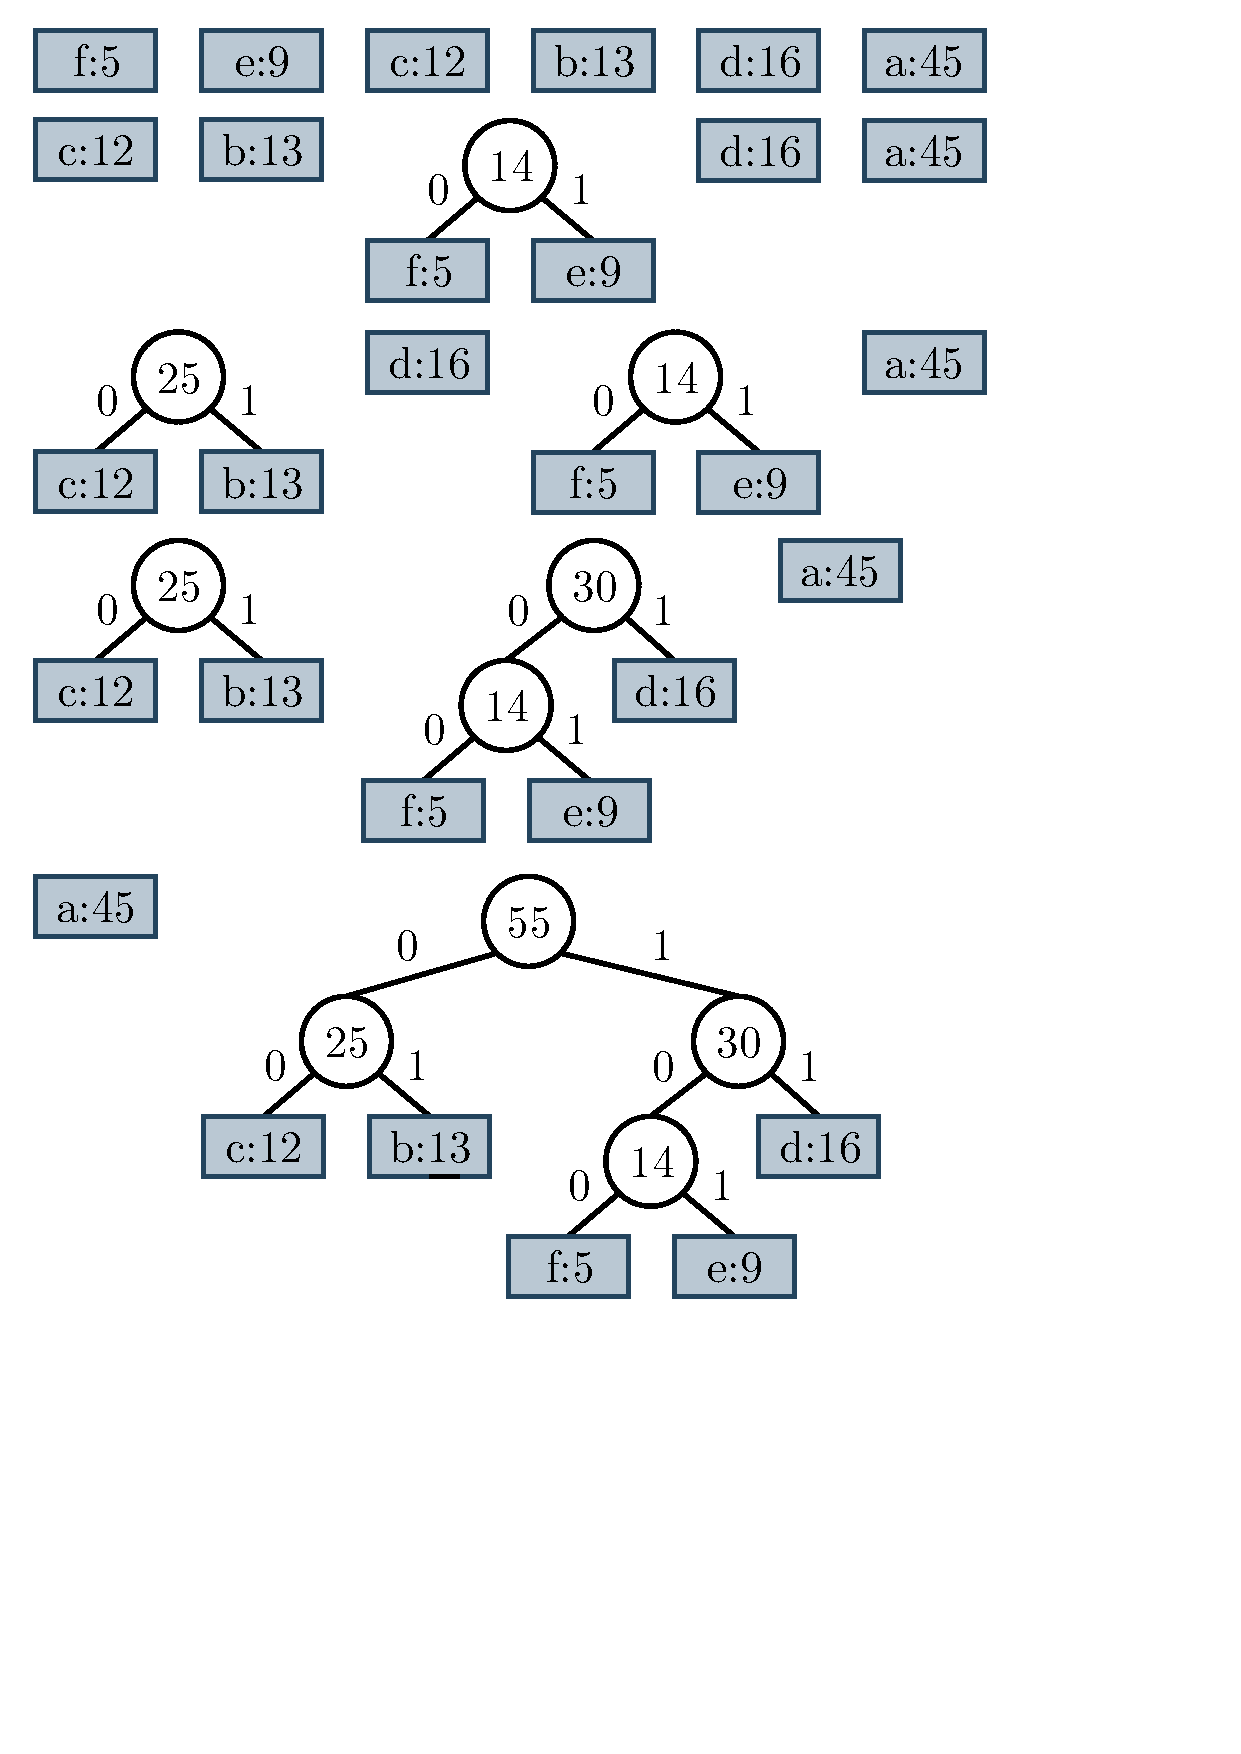
\includegraphics[scale=.4, clip, trim=10 430 160 250]{img/graphs-huffman2.pdf}
    			
    			(d)
    		\end{minipage}  
    	\end{minipage}
    	
    \begin{minipage}{1\textwidth}
    		\centering
    		\begin{minipage}{0.45\textwidth}
    			\centering
    			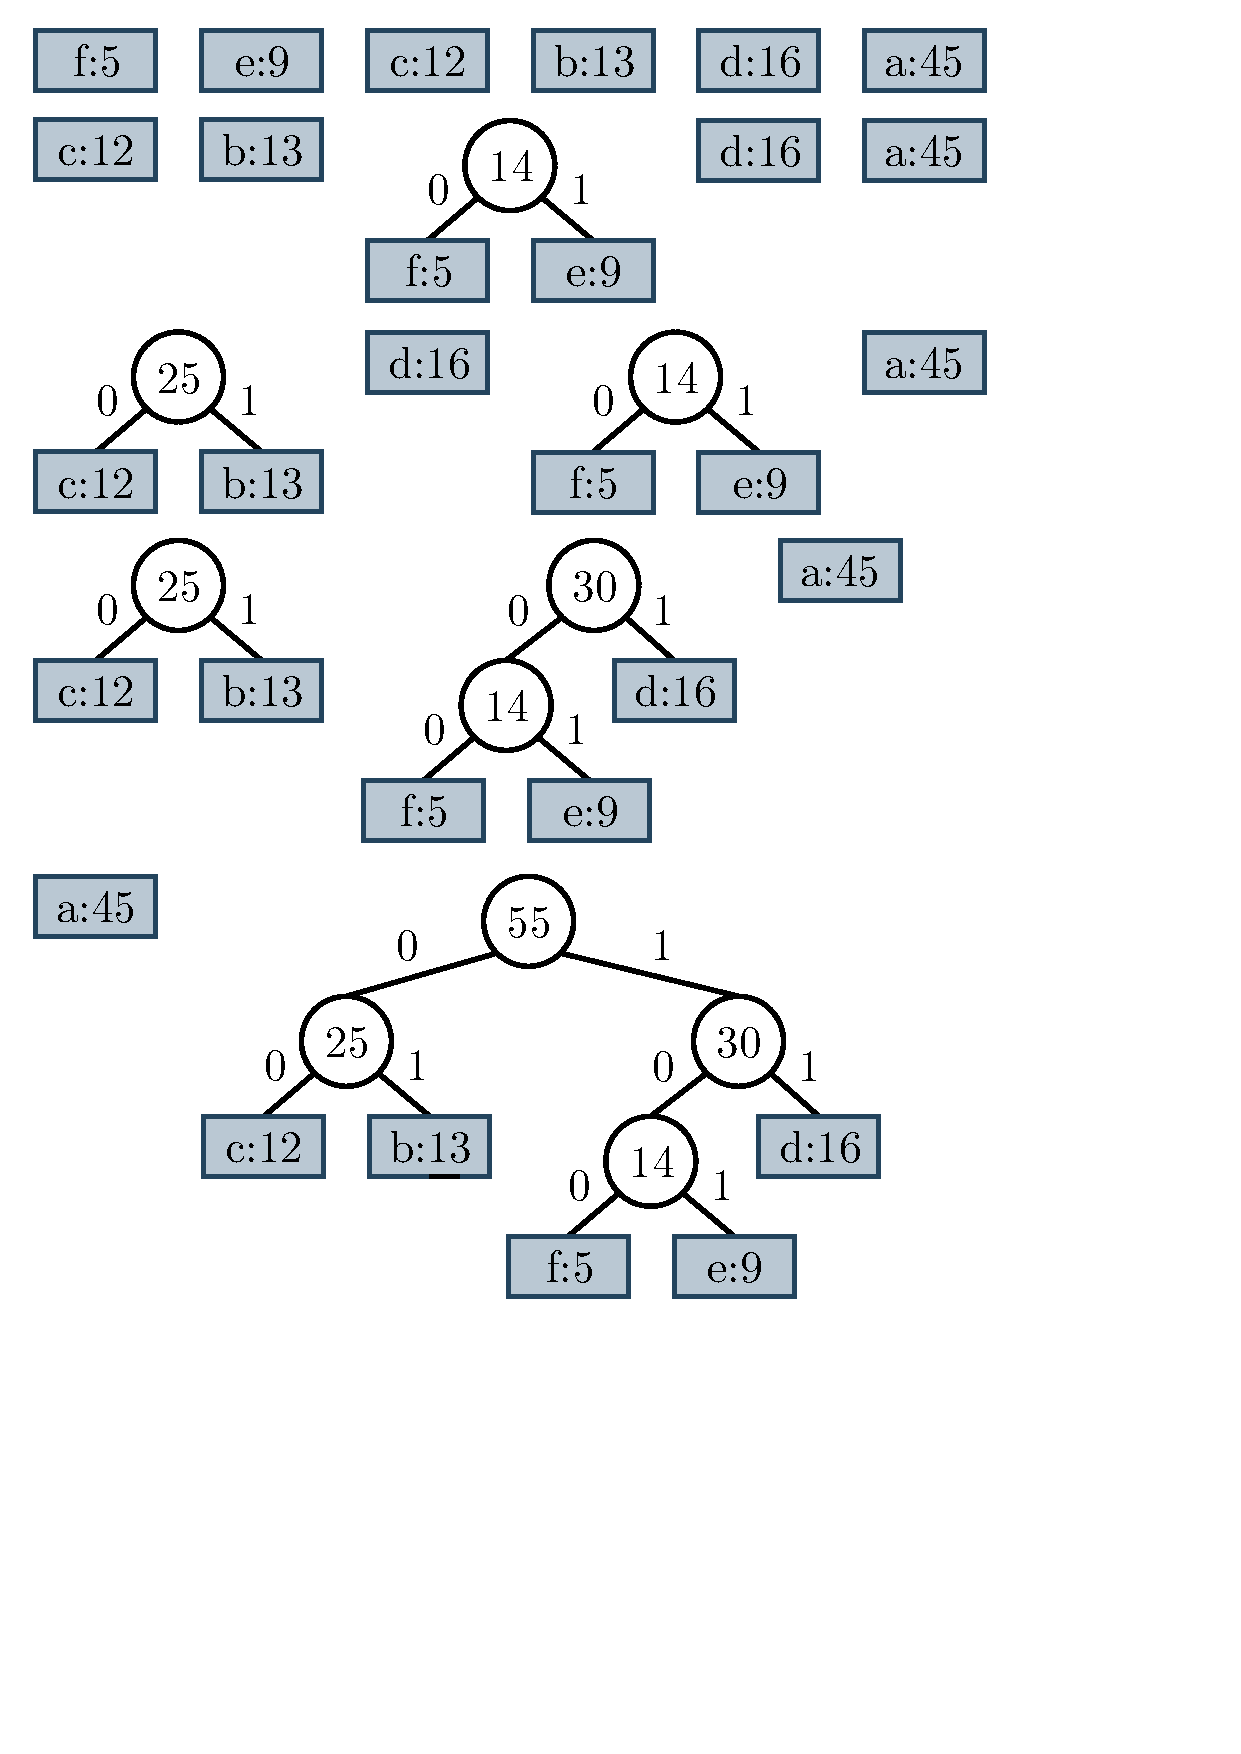
\includegraphics[scale=.4, clip, trim=10 210 170 410]{img/graphs-huffman2.pdf}
    			
    			(e)
    		\end{minipage}
    		\begin{minipage}{0.45\textwidth}
    			\centering
    			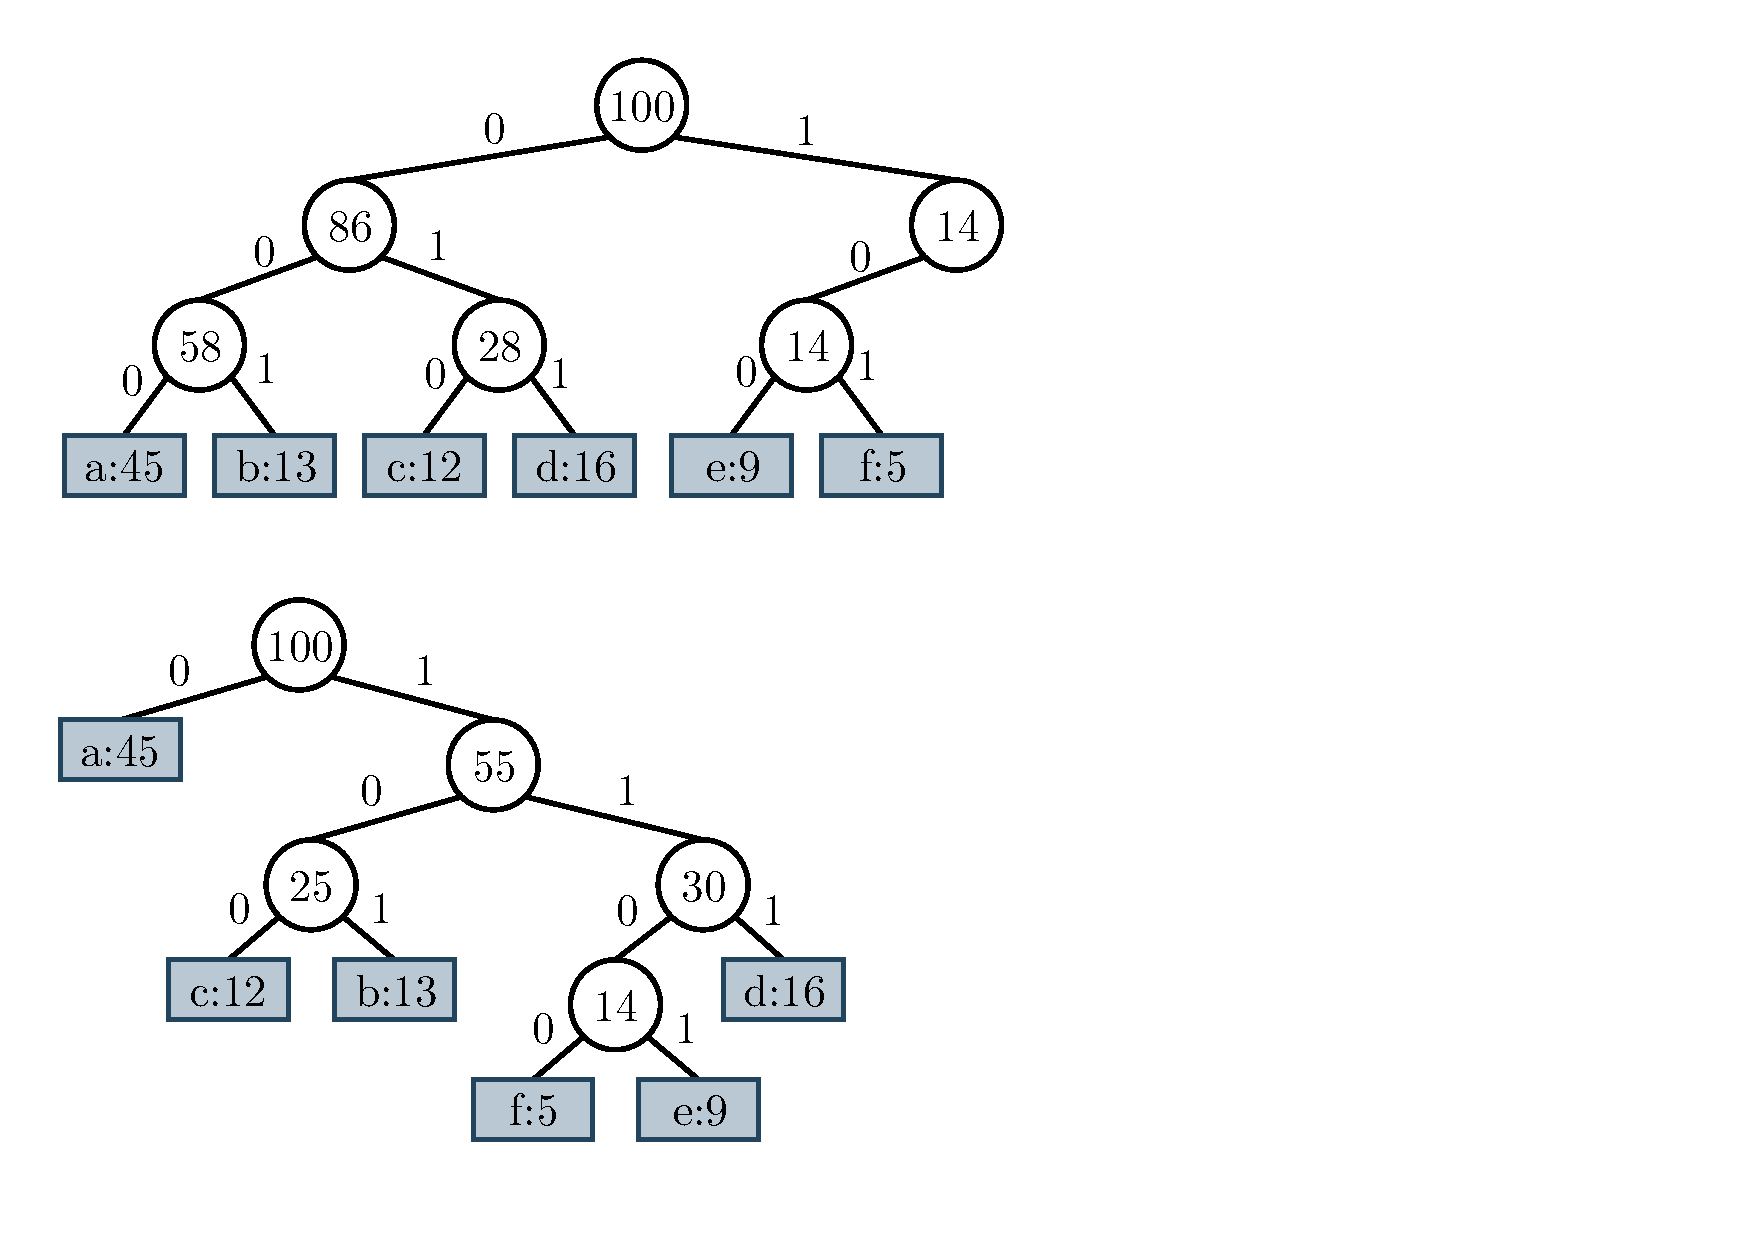
\includegraphics[scale=.4, clip, trim=20 40 430 280 ]{img/graphs-fixVarTrees.pdf}

    			(f)
    		\end{minipage}  
    	\end{minipage}
    	
    	 
    \caption{Etapas de construcción para codificación Huffman, para secuencia $C$ ejemplo. (a) Los 6 nodos hojas iniciales. (b) Primera unión. (c) Segunda unión. (c) Tercera unión. (d) Cuarta unión. (e) Quinta unión. (f) Última unión.}
    \label{fig:huffman2}
\end{figure}


\begin{figure}
    	\centering
    	\begin{minipage}{1\textwidth}
    		\centering
    		\begin{minipage}{0.45\textwidth}
    			\centering
    			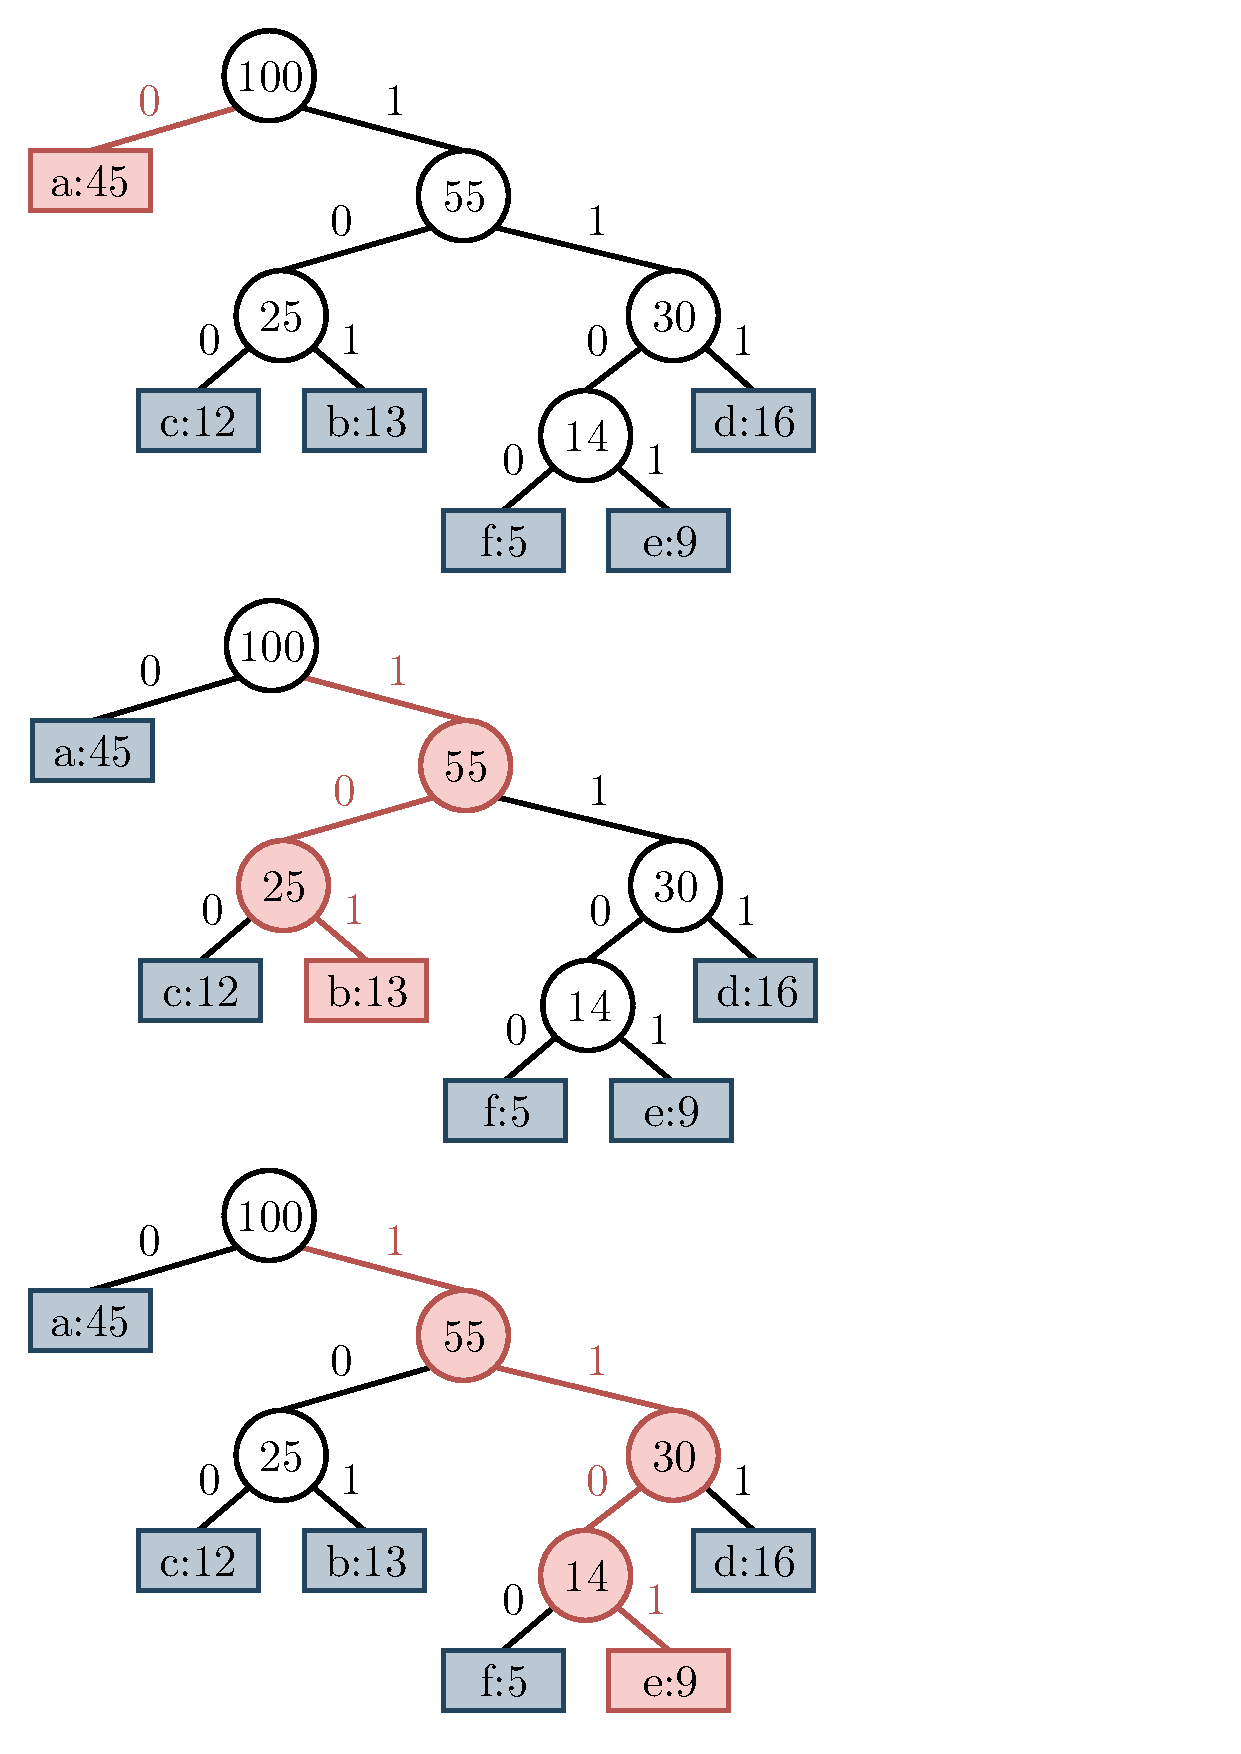
\includegraphics[scale=.45, clip, trim=10 560 200 10]{img/graphs-huffmanBack.pdf}
    			
    			(a)
    		\end{minipage}
    		\begin{minipage}{0.45\textwidth}
    			\centering
    			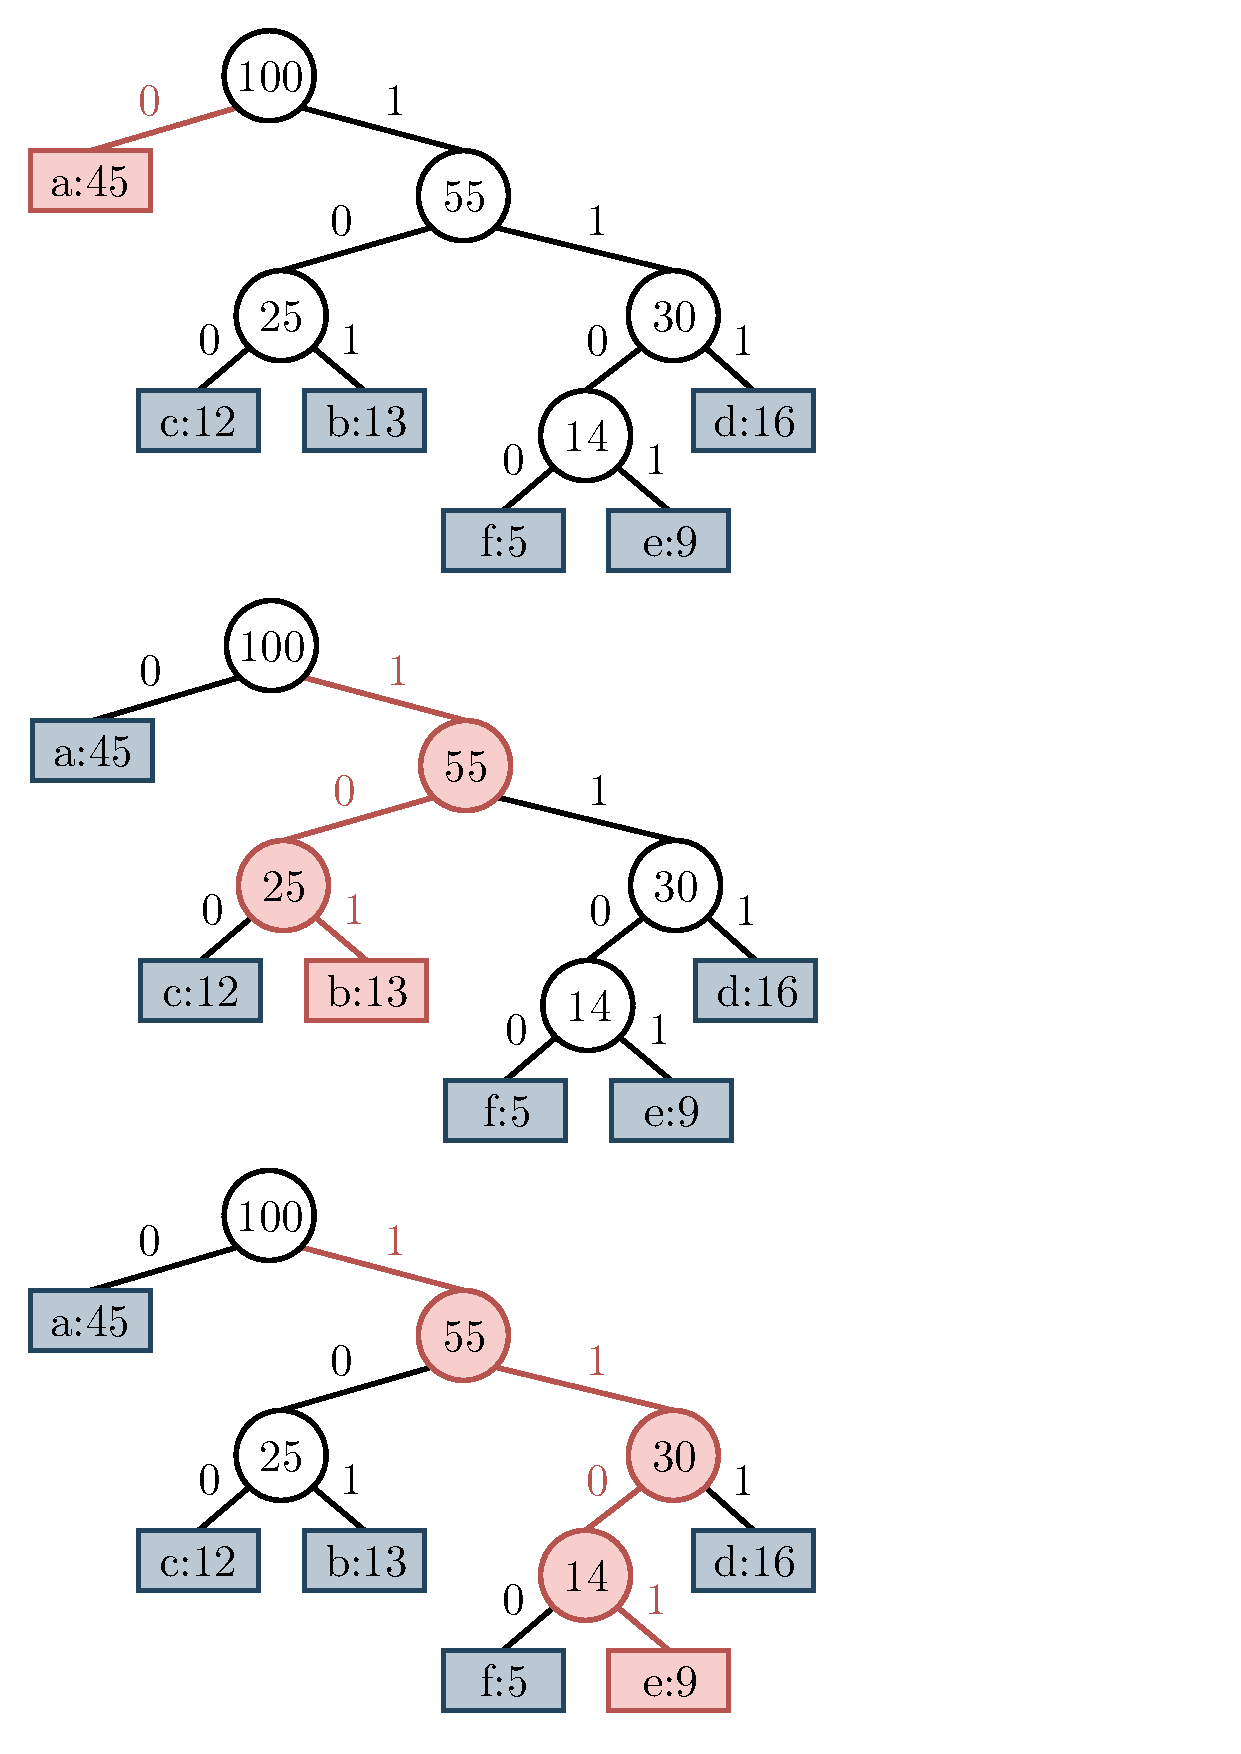
\includegraphics[scale=.45, clip, trim=10 290 200 280]{img/graphs-huffmanBack.pdf}

    			(b)
    		\end{minipage}  		
    	\end{minipage}
    	
    	\begin{minipage}{1\textwidth}
    		\centering
    		\begin{minipage}{0.45\textwidth}
    			\centering
    			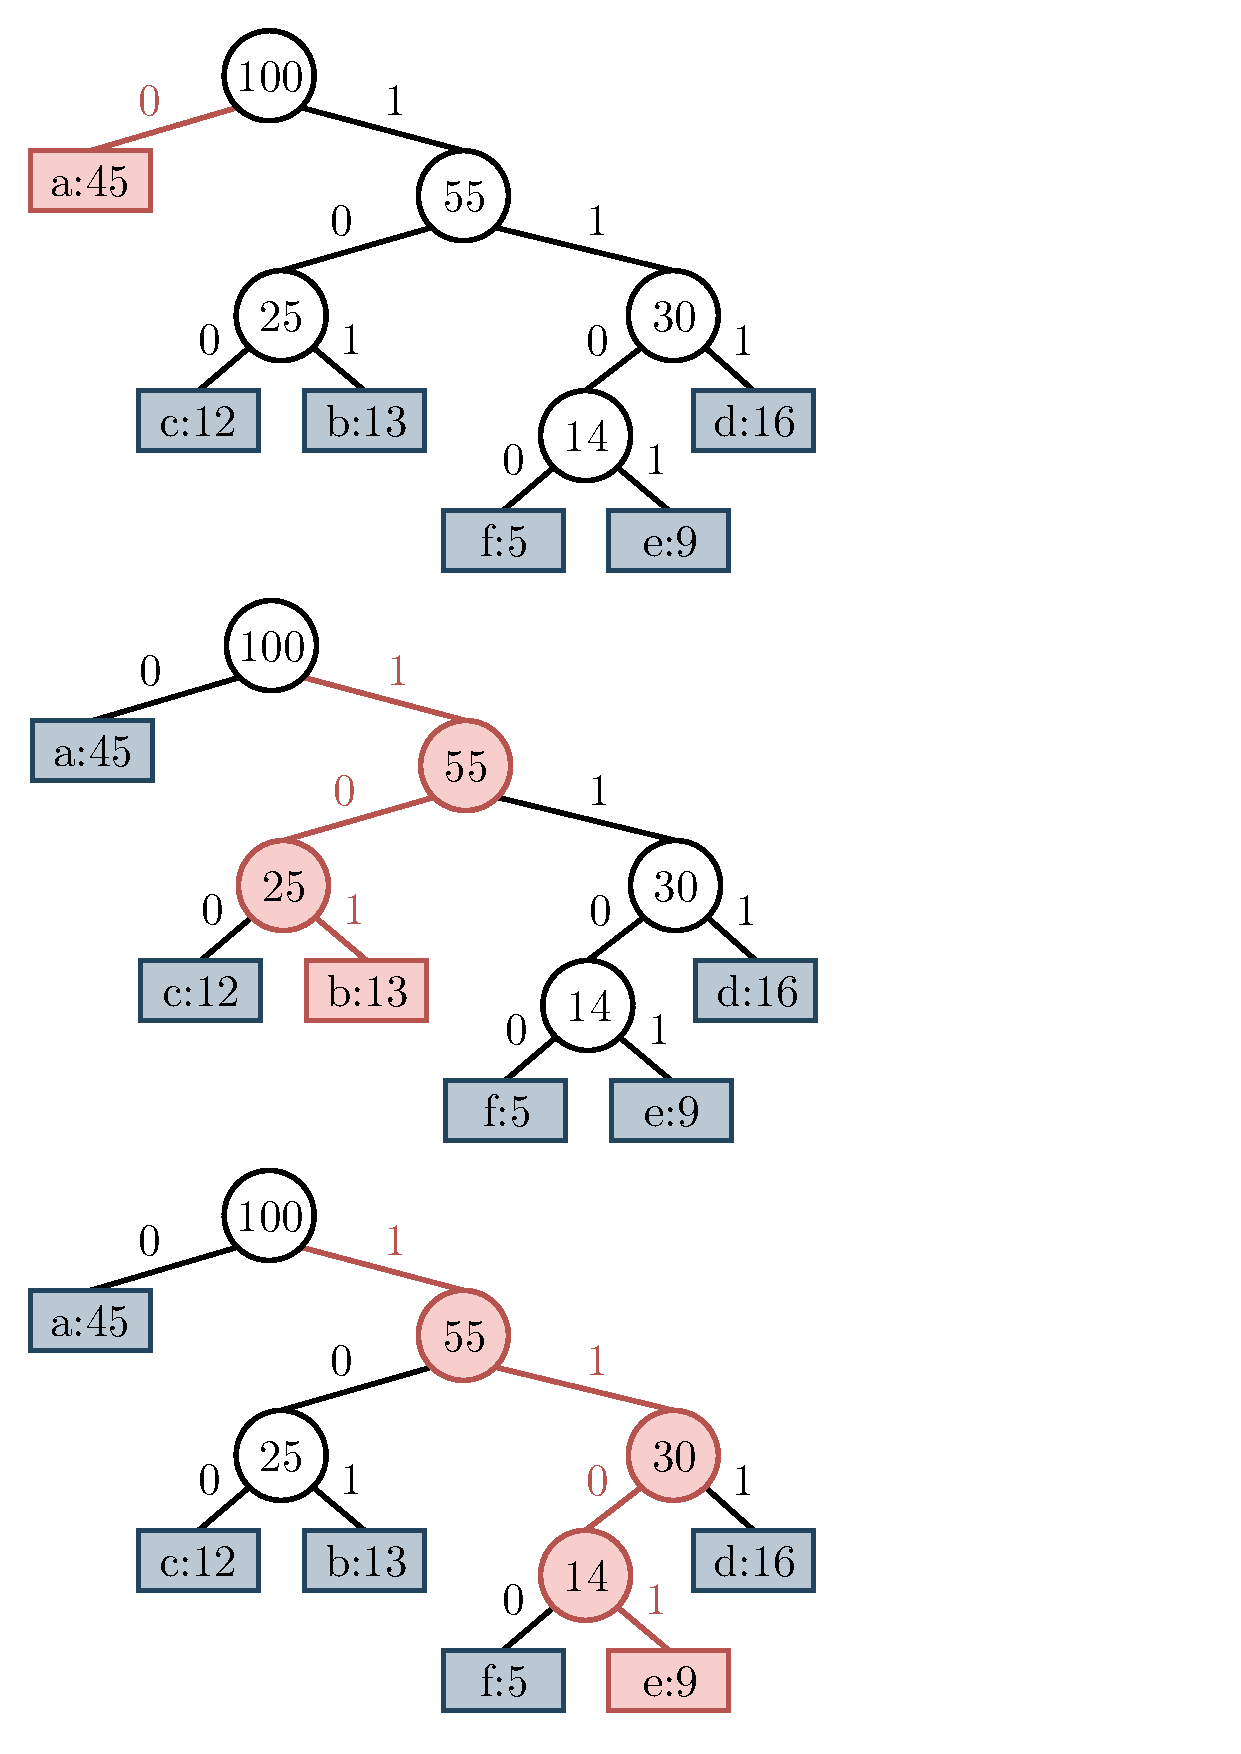
\includegraphics[scale=.4, clip, trim=10 20 200 550]{img/graphs-huffmanBack.pdf}
    			
    			(c)
    		\end{minipage}  
    		\begin{minipage}{0.45\textwidth}
    			\centering
			\begin{tabular}{cccc}
				0 & 0 & 101 & 1101 \\
				\midrule
				a & a & b & e \\
			\end{tabular}
		    	\vspace{5mm}
		    	
    			(d)
    		\end{minipage}  
    	\end{minipage}
    	
    	 
    \caption{Usando el árbol para decodificar Huffman. (a) Decodificando $0$. (b) Decodificando $101$. (c) Decodificando $1101$. (d) Equivalencias de bits y caracteres.}
    \label{fig:huffmanBack}
\end{figure}




%En la Figura~\ref{fig:huffman} se muestra un ejemplo de esta codificación, donde (a) es la secuencia de entrada, (b) es la secuencia de salida, y (c) es el vocabulario de símbolos dispuesto en un árbol binario. Primero se cuenta la frecuencia de cada símbolo en la secuencia de entrada, dos veces $1$, dos veces $2$, y cinco veces $3$. Luego se crea el árbol binario, partiendo por las hojas de los símbolos menos frecuentes, $1$ y $2$, y creando un nodo con la frecuencia total de ambos casos, en total cuatro. Luego esa rama se añade a otro nodo junto con la hoja del símbolo más probable, $3$, y ambas suman la frecuencia total de nueve símbolos. Así, el símbolo $3$ puede representarse tan solo con un bit en 1, y para los otros casos se necesitarán dos bits.
%
%
%Para recuperar la secuencia original, se debe recorrer la de salida bit a bit de izquierda a derecha, e ir avanzando en el árbol binario hasta llegar a una hoja. Una desventaja de este método es que necesita decodificar de manera secuencial todo el código para obtener la secuencia original.
